%% Draft manuscript for Springer Nature / Neural Computing and Applications style.
%% Compile on Overleaf or locally with the official Springer Nature template files:
%% sn-jnl.cls, sn-mathphys-num.bst, and related files.
%% Suggested class option for NCA-like math/engineering manuscript:
\documentclass[pdflatex,sn-mathphys-num]{sn-jnl}
\usepackage{lmodern}
\usepackage{graphicx}
\usepackage{multirow}
\usepackage{amsmath,amssymb,amsfonts}
\usepackage{amsthm}
\usepackage{mathrsfs}
\usepackage[title]{appendix}
\usepackage{xcolor}
\usepackage{textcomp}
\usepackage{manyfoot}
\usepackage{booktabs}
\usepackage{algorithm}
\usepackage{algorithmicx}
\usepackage{algpseudocode}
\usepackage{listings}
\usepackage{bm}

% \jyear{2026}

% \theoremstyle{thmstyleone}
\newtheorem{theorem}{Theorem}
\newtheorem{proposition}[theorem]{Proposition}
% \theoremstyle{thmstyletwo}
\newtheorem{example}{Example}
\newtheorem{remark}{Remark}
% \theoremstyle{thmstylethree}
\newtheorem{definition}{Definition}

\newcommand{\R}{\mathbb{R}}
\newcommand{\N}{\mathbb{N}}
\newcommand{\calG}{\mathcal{G}}
\newcommand{\calN}{\mathcal{N}}
\newcommand{\calP}{\mathcal{P}}
\newcommand{\calR}{\mathcal{R}}
\newcommand{\calT}{\mathcal{T}}
\newcommand{\calV}{\mathcal{V}}
\newcommand{\KNN}{\operatorname{KNN}}
\newcommand{\RNN}{\operatorname{RNN}}
\newcommand{\rdeg}{\operatorname{rdeg}}
\newcommand{\argmax}{\operatorname*{arg\,max}}
\newcommand{\argmin}{\operatorname*{arg\,min}}

\graphicspath{{./}{figures/}{figures/2018/}{figures/generated/}%
{figures/article_20260826/historical/}%
{figures/article_20260826/experimental/}%
{figures/article_20260826/experimental/structural_pruning/}%
{figures/article_20260826/experimental/multiscale/}%
{figures/article_20260826/experimental/gnuplot/}}

\begin{document}

\title[Round-trip KNN graph clustering]{Round-trip closure on directed k-nearest-neighbour graphs: vote kernels, multiscale clustering, and structural pruning}

\author*[1]{\fnm{Eraldo P.} \sur{Marinho}}\email{pereira.marinho@unesp.br}
\author[1]{\fnm{Caetano Mazzoni} \sur{Ranieri}}\email{cm.ranieri@unesp.br}
\author[1]{\fnm{Fabricio A.} \sur{Breve}}\email{fabricio.breve@unesp.br}

\affil*[1]{\orgdiv{Department of Statistics, Applied Mathematics and Computing},
\orgname{S\~ao Paulo State University (UNESP), Institute of Geosciences and Exact Sciences},
\orgaddress{\street{Av. 24-A, 1515}, \city{Rio Claro}, \state{S\~ao Paulo}, \country{Brazil}}}

\abstract{
We introduce a graph-based clustering formulation based on recursive, popularity-modulated, visibility-filtered round-trip closure on directed $k$-nearest-neighbour graphs, together with an optional label-free structural-pruning stage for overly connected closures. Incoming links contribute to popularity through a vote kernel, and popularity modulates a local visibility threshold in the squared-distance units used by the C implementation. We compare uniform, inverse-distance, inverse-square, and local sigmoid allocation shapes after matching every source point's outgoing vote mass to its historical inverse-square budget, while holding the unpruned closure pipeline fixed. As a software regression gate, the historical inverse-square model produced identical C and Python partitions in all 120 comparisons over eight datasets and $K=2,\ldots,16$; the subsequent kernel sweep produced 840 observations. Across 210 dataset--scale configurations, the cluster count depended on the kernel in 60 cases and the mean visible degree in all 210. The native pruning stage standardises each sufficiently large closure, compares one- through four-component diagonal Gaussian mixtures by BIC, retains only strongly supported two- or three-child graph-coherent splits, and removes their crossing visible connections. At $K=8$, it changes the variable-density result from four clusters and ARI $0.7817$ to five clusters and ARI $0.9627$. On the sparse bridge it raises ARI from $0.8083$ to $0.9853$ at $K=6$ and from $0$ to $0.9865$ at $K=10$, while leaving three already correct controls unchanged at ARI $1$. A native sensitivity check further shows that inverse-distance, inverse-square, and sigmoid allocation shapes all retain the five-cluster blobs and three-cluster bridge results; the six corresponding unpruned C partitions agree pointwise with the Python kernel definitions. An oracle-envelope comparison with seven external methods shows that pruned RTKNNC ties the perfect ARI on the standard controls, nearly matches the best Gaussian-mixture result on variable-density blobs ($0.9627$ versus $0.9639$), and obtains the highest ARI on the sparse bridge ($0.9865$, versus $0.9831$ for the nearest competitor). These results separate vote allocation, connectivity closure, and post-closure structural correction within one reproducible graph pipeline.
}

\keywords{k-nearest-neighbour graph, graph-based clustering, reverse nearest neighbours, round-trip closure, vote kernel, reverse-neighbour popularity, visibility, structural pruning, Gaussian mixture, multiscale clustering}

\maketitle


\section{Introduction}\label{sec:introduction}

Nearest-neighbour relations are among the most fundamental structures for representing finite datasets embedded in metric spaces. They occur naturally in pattern classification, nonparametric density estimation, graph construction, manifold learning, outlier detection, and clustering \citep{CoverHart1967,LoftsgaardenQuesenberry1965,Bentley1975,FriedmanBentleyFinkel1977,VonLuxburg2007}. In clustering, k-nearest-neighbour (KNN) relations have been explored through shared nearest neighbours, reciprocal nearest neighbours, mutual KNN graphs, reverse nearest-neighbour statistics, and density-based graph connectivity \citep{JarvisPatrick1973,Ertoz2003SNN,BritoChavezQuirozYukich1997,GowdaKrishna1978,ChowdhuryAmorim2018,XieLeeWangChenZhou2019}.

This paper develops a clustering formulation based on a recursive \emph{round-trip} operation in directed KNN graphs. Given a data point $x_i$, the forward step reaches one of its $K$ nearest neighbours, say $x_j\in\calN_K^+(x_i)$. The backward step then retrieves all data points that also selected $x_j$ as one of their $K$ nearest neighbours:
\begin{equation}
\calN_K^-(x_j)=\{x_\ell\in X: x_j\in\calN_K^+(x_\ell)\}.
\end{equation}
Thus, a neighbour is not used merely as a point in Euclidean space, but as an index to a reverse-neighbourhood set. This operation can be recursively applied until no additional points are reached, producing a saturated closure.

The present contribution is not the isolated use of KNN graphs, reverse nearest neighbours, or shared-neighbour similarity. Rather, it is the organisation of these elements into a popularity-modulated, visibility-filtered round-trip closure process whose evolution across $K$ values defines a multiscale cluster-layer structure. The vote kernel controls how incoming KNN links contribute to popularity; the graph construction, visibility rule, recursive expansion, singleton policy, and evaluation protocol remain fixed when kernels are compared. Because a single visible connection can otherwise join two large structures, we additionally introduce a conservative structural-pruning stage that tests large saturated closures for strong multimodal evidence and removes only the crossing visible connections of an accepted, graph-coherent split.

Recent work on KNNG-CS likewise uses distance-weighted incoming votes on a directed KNN graph to quantify local representativeness \citep{LiuEtAl2026KNNGCS}. It applies that statistic to greedy coreset selection, whereas the present contribution uses reverse-neighbour popularity inside a visibility-modulated recursive closure that produces $K$-indexed cluster layers.

\subsection{Novelty and positioning}

The novelty of the proposed method is not the isolated use of KNN graphs, reverse-neighbour sets, reverse-neighbour counts, or shared-neighbour evidence. These components are well established in the nearest-neighbour clustering literature. The contribution lies in their organisation into a recursive round-trip closure operator on directed KNN graphs, constrained by a popularity-modulated visibility rule and followed by singleton rejection. The optional enhancement then combines leadership-seeded mixture evidence with visible-graph coherence to prevent a small number of cross-structure connections from dominating the final partition. The resulting $K$-layer sequence provides a multiscale description of cluster formation, absorption, splitting, and merging without relying on a classical linkage criterion.

In this sense, the method is best understood as an algorithmic and topological construction. It does not reduce to a weighted voting rule or to a particular distance-based weight. The vote kernel is one parameterisation of the popularity mechanism inside a larger operator whose central object is the dynamics induced on the directed KNN graph: forward-neighbour selection, reverse-neighbour retrieval, popularity-modulated visibility filtering, recursive expansion, optional structural pruning, singleton rejection, and saturation.

\subsection{Main contributions}

The main contributions of this paper are as follows:
\begin{enumerate}
\item a formal round-trip operator on directed KNN graphs based on forward nearest-neighbour selection and backward reverse-neighbour retrieval;
\item a source-budget-matched family of reverse-neighbour popularity measures based on uniform, inverse-distance, inverse-square, and local sigmoid allocation shapes, with exact recovery of the historical inverse-square vote;
\item an implementation-faithful popularity-modulated RMS visibility mechanism, expressed in squared-distance units, for filtering admissible forward and backward KNN transitions;
\item a singleton-rejection rule for preventing isolated points from being reported as clusters;
\item a recursive closure process with an explicit saturation criterion;
\item an optional native structural-pruning rule that accepts only BIC-supported two- or three-child partitions satisfying minimum-size and visible-graph coherence constraints;
\item a $K$-layer representation for multiscale cluster evolution and an overlap-based diagnostic for studying cluster absorption and merging across $K$;
\item exact C--Python software regression gates, a controlled four-kernel benchmark, native pruning-sensitivity experiments, and a reproducible comparison with seven external clustering methods.
\end{enumerate}

\section{Related work}\label{sec:related}

\subsection{Shared-neighbour and Jarvis--Patrick clustering}

Jarvis and Patrick introduced a clustering criterion based on shared near neighbours \citep{JarvisPatrick1973}. Later shared-nearest-neighbour (SNN) clustering methods used common neighbour counts to improve robustness to clusters of different shapes, sizes, and densities \citep{Ertoz2003SNN}. The present method is related to this family because reverse-neighbourhood intersections imply shared-neighbour evidence. However, shared-neighbour information is not used only as a static similarity score; it is embedded in a recursive graph-closure process.

\subsection{Mutual, reciprocal, and reverse nearest-neighbour methods}

Mutual KNN and reciprocal nearest-neighbour graphs have been used for clustering and outlier detection \citep{BritoChavezQuirozYukich1997,GowdaKrishna1978,SardanaBhatnagar2014}. Reverse nearest-neighbour methods use incoming KNN links as density or representativeness signals \citep{ChowdhuryAmorim2018}. In the present formulation, reverse-neighbour sets are used both as backward adjacency relations in a round-trip closure process and as the basis for a kernel-weighted popularity measure. This popularity score modulates the local visibility threshold that controls whether a recursive forward or backward transition is admitted.

A particularly close recent construction at the level of the popularity statistic is KNNG-CS \citep{LiuEtAl2026KNNGCS}. It assigns every outgoing KNN edge a source-normalised softmax weight and defines node importance as the sum of the incoming weights. This shares with our formulation the primitive of distance-weighted reverse-neighbour popularity, but the subsequent operators and outputs are different. KNNG-CS computes node importance once, greedily selects the highest-scoring coreset representatives, and removes each selected point together with its reverse neighbours. The present method instead uses popularity to modulate visibility within a recursive forward--backward closure that produces cluster layers. Both formulations normalise the relative allocation of a source's votes, but KNNG-CS fixes the outgoing mass to one, whereas our source budget remains the geometry-dependent historical quantity $B_i=\sum_j 1/r_{ij}^2$. This preserves the original inverse-square operator exactly while allowing a controlled comparison of allocation shapes.

\subsection{Density-based and spectral graph clustering}

DBSCAN, OPTICS, and HDBSCAN define clusters through density connectivity and hierarchical density estimates \citep{Ester1996DBSCAN,Ankerst1999OPTICS,Campello2013HDBSCAN,CampelloMoulaviZimekSander2015}. Spectral clustering constructs a similarity graph and uses eigenvectors of the associated graph Laplacian to reveal cluster structure \citep{NgJordanWeiss2002,VonLuxburg2007}. The method proposed here is graph-based, but it is combinatorial and closure-driven: it does not require eigenvalue decomposition and it exposes a sequence of partitions as the neighbourhood size $K$ varies.
The comparison also includes classical agglomerative clustering
\citep{MurtaghContreras2012}, $k$-means \citep{Lloyd1982,MacQueen1967}, and
Gaussian mixtures, using the scikit-learn implementations
\citep{PedregosaEtAl2011}.

\subsection{Clustering methods for astronomical synthetic data}

The evaluation of clustering methods on structured scientific datasets is closely related to the present work. In astronomical applications, clustering may be applied not only to spatial point clouds, but also to synthetic orbital data, extracted features, and reduced-dimensional representations. Marinho et al.~\citep{PereiraMarinho2026ClusteringAO} investigated clustering methods for astronomical orbital synthetic data under feature extraction and dimensionality reduction pipelines. That work provides a complementary application context for the present paper. While the previous study emphasised the empirical behaviour of clustering methods on orbital synthetic data, the current work focuses on the graph-topological mechanism of round-trip KNN closure and on its induced multiscale partition sequence.

\section{Relational basis of the round-trip operator}\label{sec:relational_origin}

The primitive idea can be stated for an arbitrary directed relation. Let
\begin{equation}
A=\{a_1,\ldots,a_N\},\qquad B=\{b_1,\ldots,b_M\}
\end{equation}
be finite sets and let
\begin{equation}
T\subseteq A\times B
\end{equation}
be an asymmetric relation. The reflective composition induced by $T$ is
\begin{equation}
R_T=T^{-1}\circ T\subseteq A\times A.
\end{equation}
For $a\in A$, the reflective neighbourhood is
\begin{equation}
R_T(a)=T^{-1}(T(a)).
\label{eq:relational_reflection}
\end{equation}
Equation~\eqref{eq:relational_reflection} means that one first moves from $a$ to the objects related to it in $B$ and then returns to all objects in $A$ that share those objects in $B$.

For a subset $S\subseteq A$, define
\begin{equation}
R_T(S)=\bigcup_{a\in S}R_T(a).
\end{equation}
The recursive reflection is
\begin{equation}
R_T^0(S)=S,
\end{equation}
\begin{equation}
R_T^{t+1}(S)=R_T(R_T^t(S)),\qquad t\geq 0.
\label{eq:relational_iteration}
\end{equation}
The process saturates when
\begin{equation}
R_T^{s+1}(S)=R_T^s(S)
\end{equation}
for the first time. The integer $s$ is the saturation depth of $S$ under $R_T$.

This relational view provides an abstract basis for the forward--backward mechanism used by the proposed graph operator. The algorithmic construction is obtained by instantiating the relation on a directed KNN graph.

\section{Directed KNN graphs and reverse neighbourhoods}\label{sec:knn_graph}

Let
\begin{equation}
X=\{x_1,\ldots,x_N\}\subset\R^d
\end{equation}
be a finite dataset with a metric $\delta:X\times X\to\R_{\geq 0}$. For each point $x_i$, let
\begin{equation}
\calN_K^+(x_i)=\KNN_K(x_i)
\end{equation}
denote the set of its $K$ nearest proper neighbours. The directed KNN graph is
\begin{equation}
\calG_K=(X,E_K),
\end{equation}
where
\begin{equation}
(x_i,x_j)\in E_K \quad\Longleftrightarrow\quad x_j\in\calN_K^+(x_i).
\end{equation}
The reverse-neighbour set of $x_j$ is
\begin{equation}
\calN_K^-(x_j)=\RNN_K(x_j)=\{x_i\in X:x_j\in\calN_K^+(x_i)\}.
\label{eq:rnn}
\end{equation}

\begin{figure}[t]
\centering
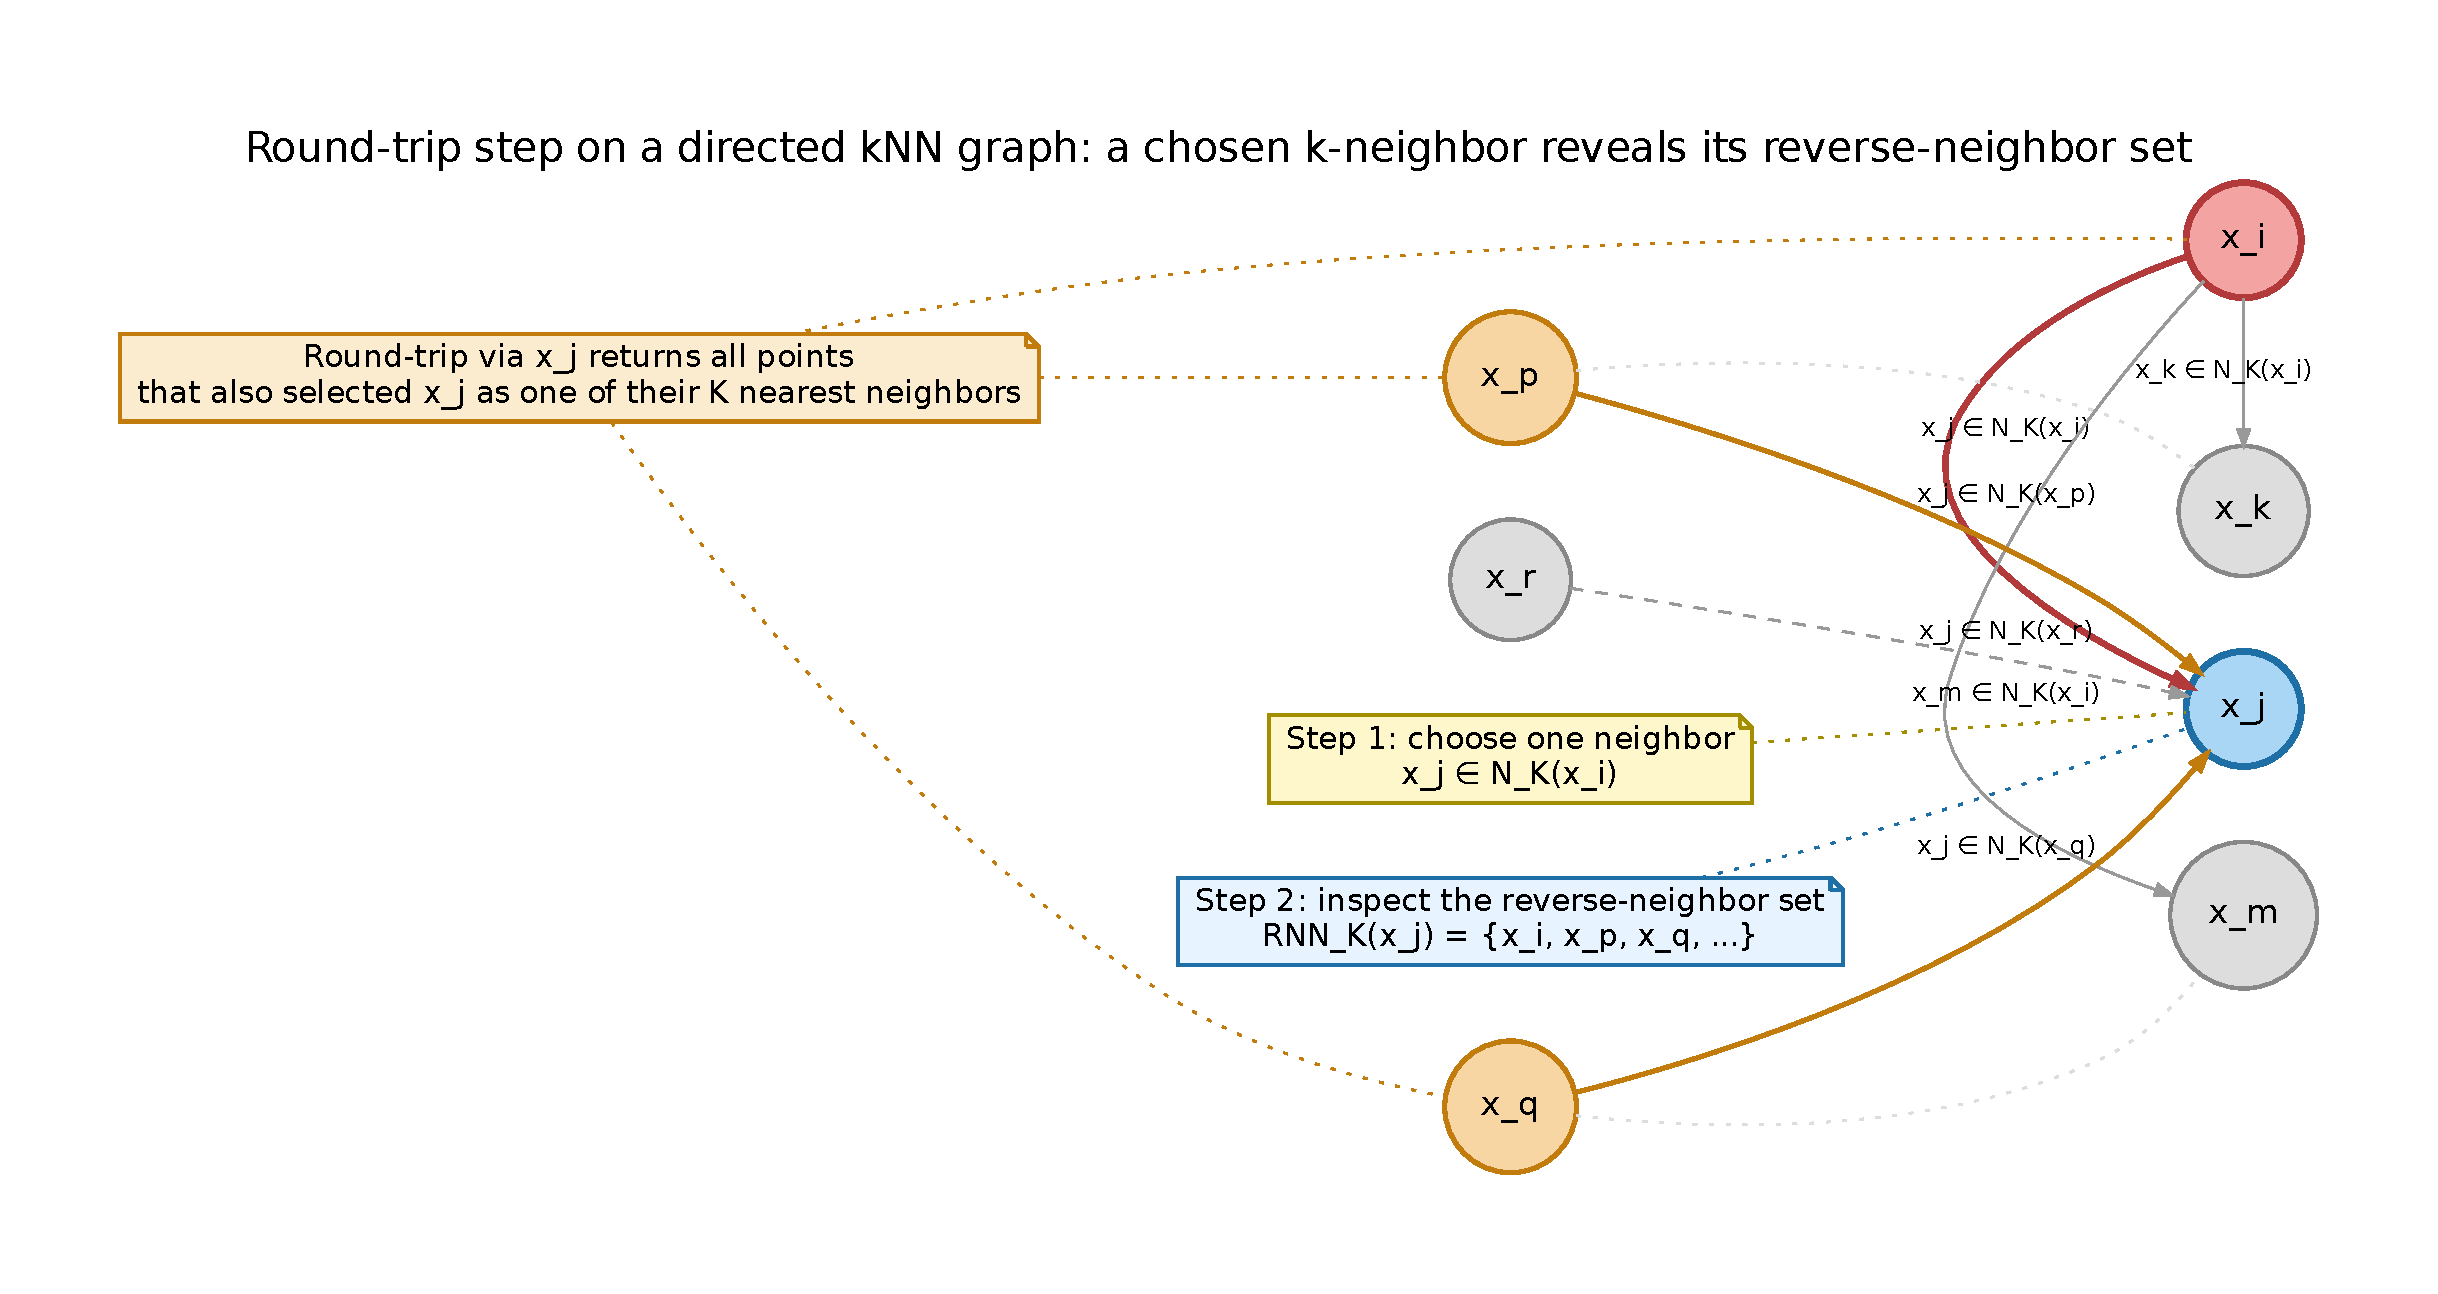
\includegraphics[width=\linewidth]{figure1_roundtrip_reverse_neighbor.pdf}
\caption{Recursive round-trip exploration on a directed KNN graph. (a) A
query point $q$ exposes its directed $K$-nearest-neighbour list and follows an
admissible transition to $p$. (b) The recursive call makes $p$ the next query,
so that $p$ exposes its own forward neighbours; the incoming purple edge
indicates that visible reverse neighbours are explored by the same routine.
(c) Every newly reached point becomes another query and the expansion repeats
until the closure no longer changes. Solid coloured arrows are traversed
transitions, whereas grey dashed arrows are KNN relations rejected by the
visibility filter.}
\label{fig:roundtrip_recursive_exploration}
\end{figure}

Figure~\ref{fig:roundtrip_recursive_exploration} shows the execution rather
than only a static reciprocal relation.  After $q$ reaches an admissible
$p\in\calV_K^+(q)$, the call on $p$ exposes $p$'s own visible forward and
backward adjacency.  Each accepted endpoint is passed to the same routine and
therefore becomes a new query.  The ``return'' in the round trip is thus an
adjacency revelation followed by recursive propagation, not a geometric
displacement back to the original point.  The process terminates when a full
pass adds no new vertices, producing the saturated closure defined in
Section~\ref{sec:visibility_closure}.

\begin{figure}[t]
\centering
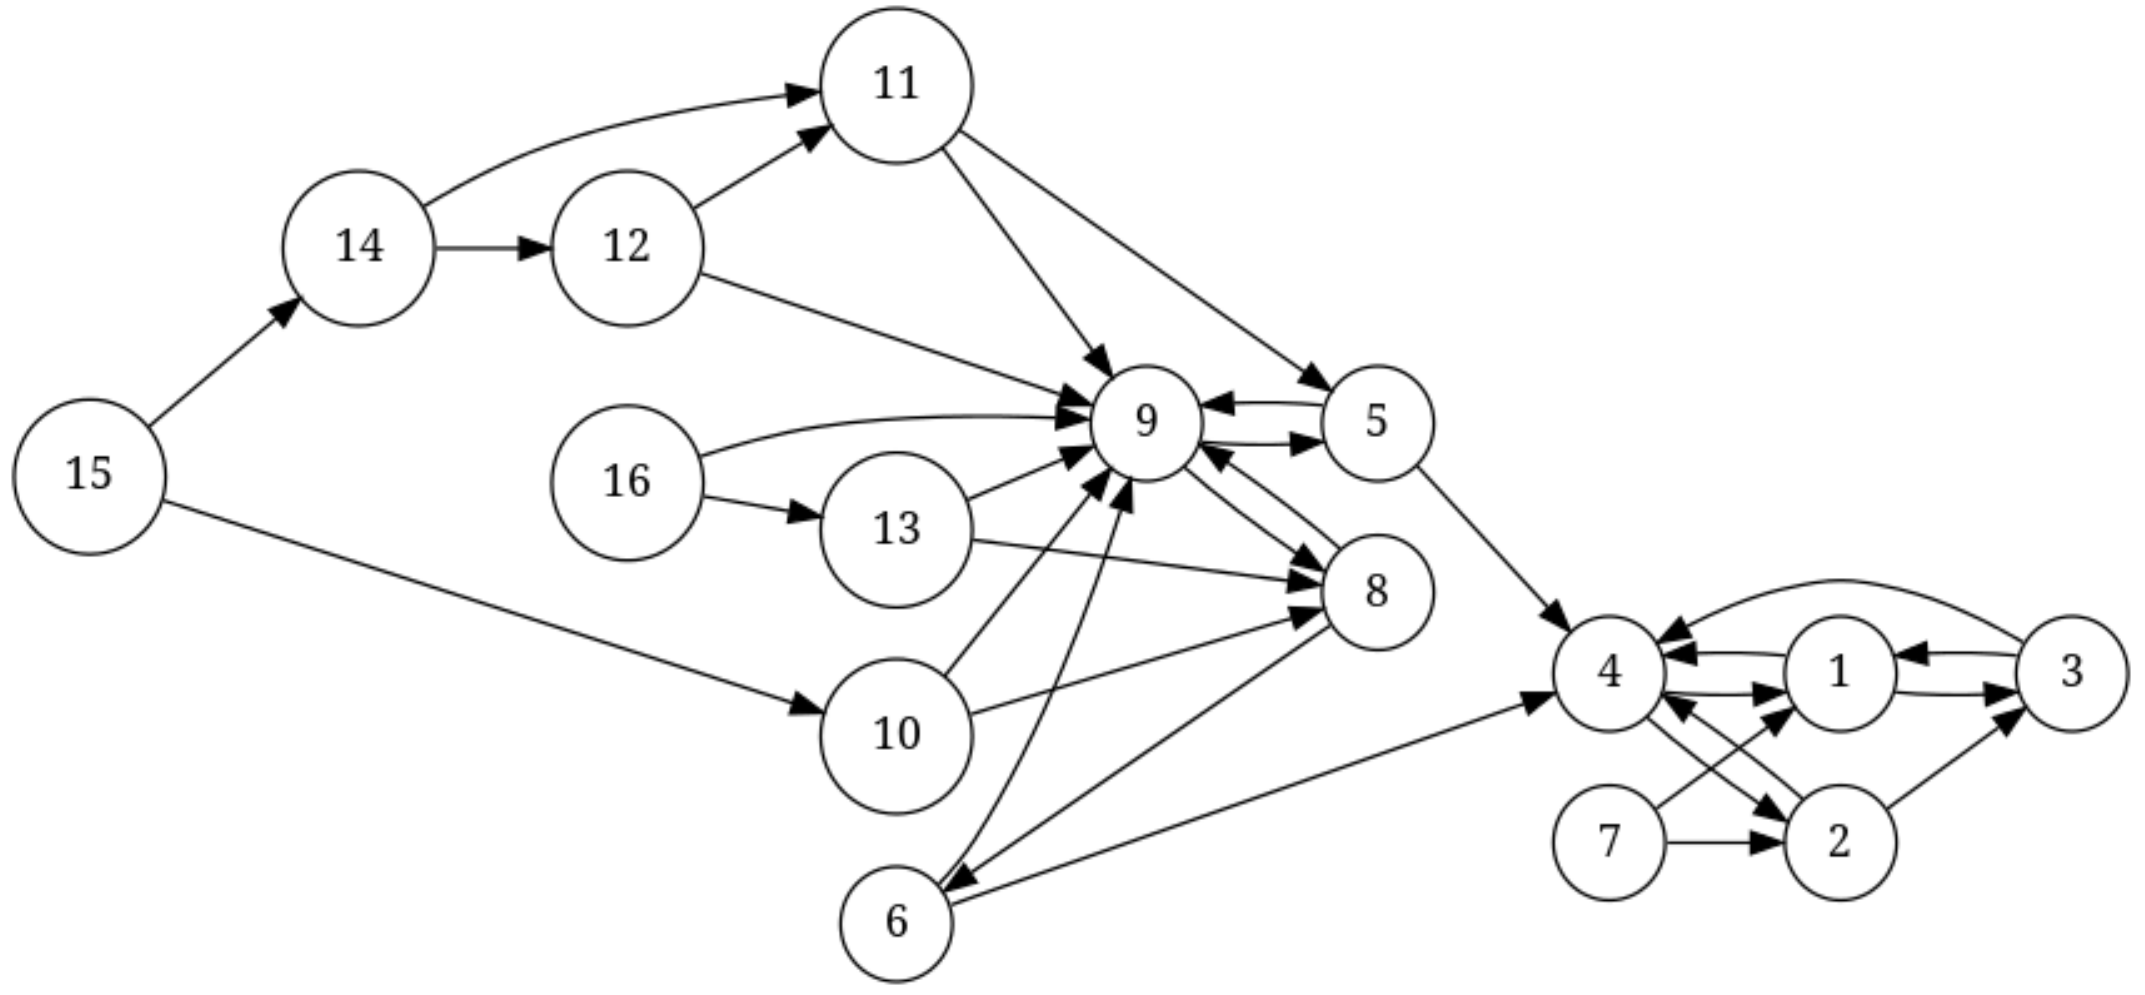
\includegraphics[width=0.78\linewidth]{fig_2018_knn_graph_black.png}
\caption{Example of a directed KNN graph used to illustrate the proposed
mechanism.  Edges represent nearest-neighbour choices and arrowheads encode
their direction.  Nodes and edges are drawn uniformly in black because the
red/blue convention in the archived rendering is undocumented and is not used
algorithmically.  The same graph supports reverse-neighbour retrieval and
visibility-filtered round-trip expansion.}
\label{fig:KNN_graph_2018}
\end{figure}

The historical prototype also organised local popularity preferences into a
leadership graph and then converted each of its weakly connected components
into a rooted tree.  Figure~\ref{fig:historical_leadership_tree} records this
provenance.  These diagrams motivate the interpretation of reverse-neighbour
popularity, but they are not an additional processing stage in the controlled
vote-kernel benchmark reported below.

\begin{figure}[t]
\centering
\begin{minipage}[c]{0.27\linewidth}
\centering
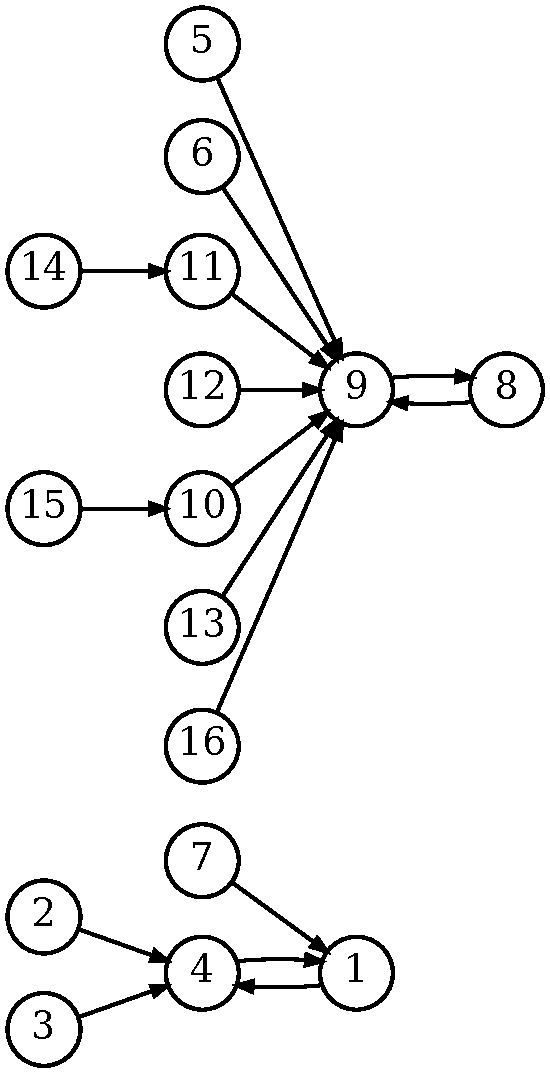
\includegraphics[width=\linewidth]{fig_2018_leadership_graph_black.pdf}
\par\smallskip
{\footnotesize (a) directed leadership graph}
\end{minipage}
\hfill
\begin{minipage}[c]{0.10\linewidth}
\centering
{\scriptsize break\\2-cycles}\par
\smallskip
{\Large$\Longrightarrow$}\par
\smallskip
{\scriptsize orient from\\the roots}
\end{minipage}
\hfill
\begin{minipage}[c]{0.57\linewidth}
\centering
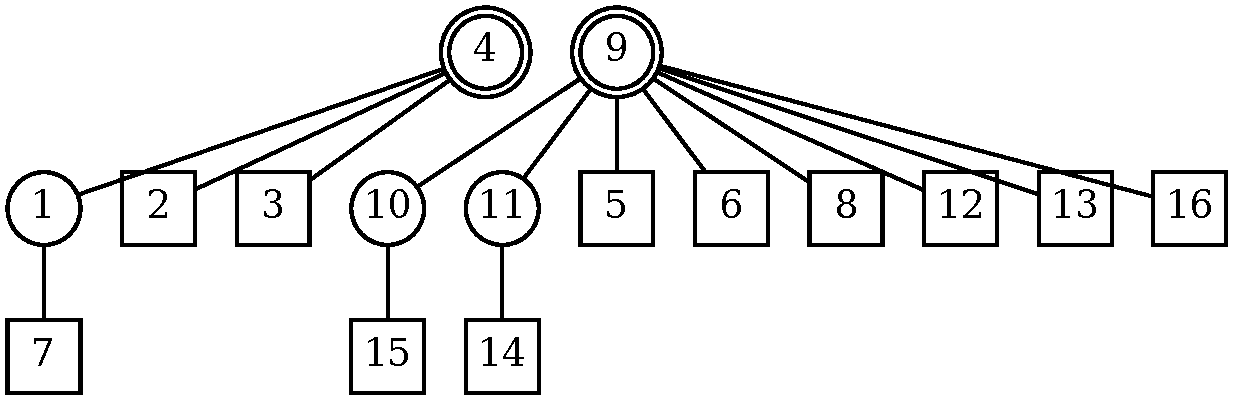
\includegraphics[width=\linewidth]{fig_2018_cluster_forest_corrected.pdf}
\par\smallskip
{\footnotesize (b) rooted leadership forest}
\end{minipage}
\caption{From the historical leadership graph to its rooted forest for the
same 16-point KNN example.  In (a), every vertex points to its locally selected
leader; the graph has two weakly connected components, each containing a
reciprocal leader pair, $1\leftrightarrow4$ and $8\leftrightarrow9$.  Resolving
each pair at its more popular vertex and displaying parent--child links away
from roots 4 and 9 produces the two trees in (b).  Vertex identifiers are
preserved across panels, while nodes and edges are drawn uniformly in black so
that colour carries no undocumented semantics.  Double circles mark roots,
single circles internal leaders, and squares leaves.}
\label{fig:historical_leadership_tree}
\end{figure}

\section{Vote-kernel popularity, visibility, and round-trip closure}\label{sec:visibility_closure}

The reference formulation adopts a popularity-modulated, visibility-filtered round-trip expansion. A point need not propagate through all of its $K$ nearest-neighbour links: only links admitted by its local visibility threshold participate in the forward--backward closure. To reproduce the reference implementation exactly, linear and squared distances must be distinguished.

\subsection{Distance representation and legacy radius}

Let
\begin{equation}
r_{ij}=\delta(x_i,x_j),
\qquad
D_{ij}=r_{ij}^{2}.
\label{eq:linear_squared_distance}
\end{equation}
The C implementation stores $D_{ij}$, rather than $r_{ij}$, in each KNN list. After the list is sorted, its stored radius is the largest retained squared distance,
\begin{equation}
R_K^{(2)}(x_i)=D_{i,(K)}
=\max_{x_j\in\calN_K^+(x_i)}D_{ij}.
\label{eq:legacy_radius}
\end{equation}
The corresponding linear scale is
\begin{equation}
R_K(x_i)=\sqrt{R_K^{(2)}(x_i)}=r_{i,(K)}.
\label{eq:linear_knn_radius}
\end{equation}

\subsection{Vote kernels and reverse-neighbour popularity}

For each source point $x_i$, define the dimensionless neighbour coordinate
\begin{equation}
u_{ij}=\frac{r_{ij}}{R_K(x_i)},
\qquad x_j\in\calN_K^+(x_i),
\label{eq:normalised_neighbour_distance}
\end{equation}
and compare the four allocation shapes
\begin{equation}
h(u)\in
\left\{
1,\frac{1}{u},\frac{1}{u^2},S_\alpha(u)
\right\},
\label{eq:vote_kernel_family}
\end{equation}
where
\begin{equation}
S_\alpha(u)=\frac{1}{1+\exp[\alpha(u-1)]}.
\label{eq:sigmoid_vote}
\end{equation}
Here, $\alpha>0$ controls the slope, and $R_K(x_i)$ supplies the local distance scale for every shape.  Directly comparing the raw values $1$, $1/r$, $1/r^2$, and $S_\alpha(r/R_i)$ would confound shape with units and arbitrary outgoing amplitude.  We therefore retain the historical inverse-square vote mass of source $i$ as the common budget
\begin{equation}
B_K(x_i)=\sum_{x_k\in\calN_K^+(x_i)}\frac{1}{r_{ik}^2},
\label{eq:historical_source_budget}
\end{equation}
and redistribute that budget according to the selected shape:
\begin{equation}
g_{i,h}(x_j)=B_K(x_i)
\frac{h(u_{ij})}
{\displaystyle\sum_{x_k\in\calN_K^+(x_i)}h(u_{ik})}.
\label{eq:budget_matched_vote}
\end{equation}
Thus $\sum_j g_{i,h}(x_j)=B_K(x_i)$ for every model, and the incoming popularity of $x_j$ is
\begin{equation}
P_{K,g}(x_j)=
\sum_{x_i:\,x_j\in\calN_K^+(x_i)}g_{i,h}(x_j).
\label{eq:reverse_popularity}
\end{equation}
For $h(u)=1/u^2$, Eq.~\eqref{eq:budget_matched_vote} reduces algebraically to the historical edge vote,
\begin{equation}
g_{i,\mathrm{inv}\_r2}(x_j)
=B_K(x_i)\frac{(R_K(x_i)/r_{ij})^2}
{\sum_{x_k\in\calN_K^+(x_i)}(R_K(x_i)/r_{ik})^2}
=\frac{1}{r_{ij}^2}=\frac{1}{D_{ij}}.
\label{eq:historical_reverse_popularity}
\end{equation}
The implementation uses this final expression directly for the inverse-square branch, avoiding a normalise--denormalise round-off cycle. Exact duplicate observations are excluded because the shared historical budget is undefined at $r=0$.

\subsection{RMS visibility in squared-distance units}

The unmodulated visibility threshold is the RMS of the stored squared distances,
\begin{equation}
V_{K,0}^{(2)}(x_i)=
\left(
\frac{1}{K}
\sum_{x_j\in\calN_K^+(x_i)}D_{ij}^{2}
\right)^{1/2}.
\label{eq:rms_visibility_base}
\end{equation}
Popularity then produces the effective threshold
\begin{equation}
V_{K,g}^{(2)}(x_i)=V_{K,0}^{(2)}(x_i)
\left(1+\frac{P_{K,g}(x_i)R_K^{(2)}(x_i)}{N}\right).
\label{eq:popularity_modulated_visibility}
\end{equation}
Equations~\eqref{eq:historical_reverse_popularity}--\eqref{eq:popularity_modulated_visibility} reproduce the historical inverse-square implementation exactly. The comparison models change only the within-source allocation in Eq.~\eqref{eq:budget_matched_vote}. Under a global coordinate rescaling $r\mapsto cr$, all four vote families scale as $c^{-2}$ because $B_K\mapsto c^{-2}B_K$, while $R_K^{(2)}\mapsto c^2R_K^{(2)}$; hence the popularity factor $P_{K,g}R_K^{(2)}$ is invariant for every model. Feature-wise preprocessing can still change the KNN graph and must therefore be specified and reused exactly.

\subsection{Visible forward and backward steps}

The visible forward neighbourhood of $x_i$ is
\begin{equation}
\calV_K^+(x_i)=
\{x_j\in\calN_K^+(x_i):D_{ij}\leq V_{K,g}^{(2)}(x_i)\}.
\label{eq:visible_forward}
\end{equation}
The visible backward neighbourhood of $x_i$ is
\begin{equation}
\calV_K^-(x_i)=
\{x_\ell\in\calN_K^-(x_i):D_{\ell i}\leq V_{K,g}^{(2)}(x_\ell)\}.
\label{eq:visible_backward}
\end{equation}
The backward condition is evaluated from the viewpoint of the reverse neighbour $x_\ell$: a reverse-neighbour step is accepted only if $D_{\ell i}$ does not exceed the squared-distance visibility threshold of $x_\ell$. The one-step visibility-filtered round-trip neighbourhood is therefore
\begin{equation}
\calR_K^{\mathrm{vis}}(x_i)=\calV_K^+(x_i)\cup\calV_K^-(x_i).
\label{eq:visible_roundtrip}
\end{equation}

\subsection{Recursive closure and singleton rejection}

Starting from a seed point $x_i$, the recursive closure is
\begin{equation}
C_K^0(x_i)=\{x_i\},
\end{equation}
\begin{equation}
C_K^{t+1}(x_i)=C_K^t(x_i)\cup
\bigcup_{x_q\in C_K^t(x_i)}\calR_K^{\mathrm{vis}}(x_q).
\label{eq:visibility_closure}
\end{equation}
The process saturates when
\begin{equation}
C_K^{t+1}(x_i)=C_K^t(x_i).
\end{equation}
The saturated closure is denoted
\begin{equation}
C_K^\infty(x_i)=C_K^s(x_i),
\end{equation}
where $s$ is the first saturation time.

A saturated closure is accepted as a cluster only when it contains more than one point:
\begin{equation}
|C_K^\infty(x_i)|>1.
\label{eq:singleton_rejection}
\end{equation}
This singleton-rejection rule prevents isolated points or failed expansions from being reported as meaningful clusters. In the reported synthetic experiments, the accepted layers are subsequently checked to verify whether they cover the full dataset and therefore form proper partitions.

\begin{algorithm}[t]
\caption{Visibility-filtered round-trip closure for one point}
\label{alg:visibility_closure}
\begin{algorithmic}[1]
\Require directed KNN graph $\calG_K$, vote model $g$, visibility thresholds $V_{K,g}^{(2)}$, point $x_i$
\State $C \gets \{x_i\}$
\Repeat
    \State $C_{old}\gets C$
    \ForAll{$x_q\in C_{old}$}
        \State $C\gets C\cup\calV_K^+(x_q)$
        \State $C\gets C\cup\calV_K^-(x_q)$
    \EndFor
\Until{$C=C_{old}$}
\If{$|C|>1$}
    \State \Return $C$
\Else
    \State \Return rejected singleton closure
\EndIf
\end{algorithmic}
\end{algorithm}

\subsection{Optional structural pruning of saturated closures}
\label{sec:structural_pruning}

The baseline closure has an intentionally strong connectivity semantics: one
visible path is sufficient to join its endpoints.  Structural pruning is an
optional second stage, enabled in the native executable by
\texttt{--structural-pruning}, that tests whether a large baseline component
contains strongly supported internal populations.  It is disabled by default,
so the historical inverse-square regression and the four-kernel ablation remain
unchanged.  The native selector \texttt{--vote-kernel} accepts
\texttt{uniform}, \texttt{inv\_r}, \texttt{inv\_r2}, or \texttt{sigmoid};
\texttt{inv\_r2} remains the default, and the sigmoid slope is controlled by
\texttt{--sigmoid-alpha} (default $8$).  The selected kernel supplies both the
popularity-modulated visible graph and the popularity-ranked first mixture
seed, while every subsequent pruning criterion is held fixed.

Let $C$ be a baseline closure.  It is considered for pruning only when
\begin{equation}
|C|\geq n_{\mathrm{parent}}
=\max\{50,\lceil0.15N\rceil\}.
\label{eq:pruning_parent_size}
\end{equation}
Each coordinate is standardised within $C$, and diagonal-covariance Gaussian
mixtures with $m\in\{1,2,3,4\}$ components are fitted by expectation--maximisation
\citep{DempsterLairdRubin1977}.  For dimension $d$, the implementation compares
\begin{equation}
\operatorname{BIC}_m=-2\ell_m+p_m\log |C|,
\qquad p_m=m(2d+1)-1,
\label{eq:pruning_bic}
\end{equation}
where $\ell_m$ is the maximised log likelihood and $p_m$ counts mixture
weights, means, and diagonal variances \citep{Schwarz1978}.  Models with
$m>1$ use five deterministic restarts.  In the first restart, the initial
centre is the point of greatest reverse-neighbour popularity and subsequent
centres are chosen by farthest-first traversal; this is the operational role
of leadership in the pruning stage.  The remaining restarts use deterministic
seeds, making repeated executions reproducible.

Let $m^*=\argmin_m\operatorname{BIC}_m$.  A candidate is retained only if
\begin{equation}
m^*\in\{2,3\},\qquad
\operatorname{BIC}_1-\operatorname{BIC}_{m^*}\geq10,
\label{eq:pruning_acceptance}
\end{equation}
and every proposed child contains at least
\begin{equation}
n_{\mathrm{child}}=
\max\{20,\lceil0.05|C|\rceil\}
\label{eq:pruning_child_size}
\end{equation}
points.  Thus, a four-component optimum is a conservative veto rather than an
instruction to subdivide a curved or extensively fragmented closure.

Mixture membership alone does not determine the output.  Each proposed child
must also be coherent in the symmetrised visible KNN graph.  A fragment smaller
than $n_{\mathrm{child}}$ is reassigned to the alternative child with the
greatest visible-edge support; the proposal is rejected if a child retains
multiple large fragments or if a size constraint fails after regularisation.
For an accepted labelling $z_C$, the crossing set is
\begin{equation}
E_C^{\mathrm{cut}}=
\left\{\{i,j\}\in\overline E_{K,g}^{\mathrm{vis}}[C]:
z_C(i)\neq z_C(j)\right\},
\label{eq:pruning_cut}
\end{equation}
where $\overline E_{K,g}^{\mathrm{vis}}$ denotes the visible graph after
disregarding edge orientation.  The split is applied only when
$|E_C^{\mathrm{cut}}|>0$; its regularised children replace $C$ in the final
layer.  Equivalently, this removes the accepted crossing visible connections
before the component labels are rebuilt.  Reference labels play no role in
proposal generation, model selection, regularisation, or edge pruning.

\section{Cluster layers and multiscale evolution}\label{sec:layers}

For a fixed $K$, the accepted saturated closures define a cluster layer
\begin{equation}
\calP_K=\{C_1^{(K)},\ldots,C_{m_K}^{(K)}\}.
\end{equation}
By varying $K$ over a prescribed set of scales
\begin{equation}
K\in\{K_{\min},K_{\min}+1,\ldots,K_{\max}\},
\end{equation}
one obtains a multiscale sequence
\begin{equation}
\calP_{K_{\min}},\calP_{K_{\min}+1},\ldots,\calP_{K_{\max}}.
\end{equation}
In the controlled experiments, each layer is an independent execution:
$\calG_K$, $R_K^{(2)}$, popularity, and visibility are constructed for that
same value of $K$ by invoking the supported interface with $K_0=K$.  This is an
explicit experimental convention, not a claim that the intermediate layers of
one raw $K_0\!<\!K_{\max}$ process are numerically identical.  In the latter
mode, the neighbour list is allocated at $K_{\max}$ before the internal loop,
so a stored construction-time radius may remain tied to $K_{\max}$ at its
smaller layers.  Independent execution makes every reported $\calP_K$ a
function of one stated neighbourhood scale and prevents this second scale from
being implicit.

Increasing $K$ tends to increase graph connectivity. Therefore, small clusters from lower-$K$ layers are expected to be absorbed into larger clusters at higher $K$ values, although the exact behaviour depends on the dataset and on the visibility rule.

\subsection{Inter-layer overlap}

The overlap between clusters in consecutive layers is
\begin{equation}
W_{ab}^{(K,K')}=|C_a^{(K)}\cap C_b^{(K')}|.
\label{eq:overlap_count}
\end{equation}
Useful normalisations include
\begin{equation}
F_{ab}^{(K,K')}=\frac{|C_a^{(K)}\cap C_b^{(K')}|}{|C_a^{(K)}|},
\label{eq:frac_from}
\end{equation}
and the Jaccard index
\begin{equation}
J_{ab}^{(K,K')}=\frac{|C_a^{(K)}\cap C_b^{(K')}|}{|C_a^{(K)}\cup C_b^{(K')}|}.
\label{eq:jaccard}
\end{equation}

Inter-layer overlap is expected and informative: it describes how clusters from one scale are preserved, absorbed, or merged at another scale. This is distinct from intra-layer overlap, which would indicate that a given layer is not a proper partition.

\subsection{Saturation scale}

A beneficial side effect of the $K$-layer construction is that the neighbourhood scale can be selected from the saturation behaviour of the induced cluster-layer sequence. We denote by $K_{\mathrm{sat}}$ the first value of $K$ for which the accepted layer becomes stable under further increases of the neighbourhood size, up to relabelling of cluster indices. Lower values of $K$ often expose local fluctuations, microfragmentation, or noise-like components, whereas the saturated layer represents the dominant macro-scale aggregation structure.

Operationally, saturation can be detected by monitoring the overlap between consecutive layers. If each cluster in $\calP_K$ maps entirely to a unique cluster in $\calP_{K+1}$, and vice versa, the two layers are equivalent. More robustly, one may require the same equivalence to persist over a short stability window,
\begin{equation}
\calP_K \equiv \calP_{K+1}\equiv\cdots\equiv\calP_{K+h},
\label{eq:partition_stability_window}
\end{equation}
where $h$ is a prescribed persistence parameter. The saturation scale can then be defined as
\begin{equation}
K_{\mathrm{sat}}=
\min\left\{
K:\calP_K \equiv \calP_{K+1}\equiv\cdots\equiv\calP_{K+h}
\right\}.
\label{eq:ksat}
\end{equation}
Here, $\equiv$ denotes equality of cluster layers up to relabelling of cluster indices.

\section{Implementation agreement and partition diagnostic}\label{sec:partition_diagnostic}

An important consistency check is whether each accepted layer $\calP_K$ is a true partition of the dataset. For each $K$, this can be verified by comparing the sum of accepted cluster cardinalities with the cardinality of the union of all accepted cluster members:
\begin{equation}
\sum_{a=1}^{m_K}|C_a^{(K)}|=\left|\bigcup_{a=1}^{m_K}C_a^{(K)}\right|.
\label{eq:partition_check}
\end{equation}
When the equality in Eq.~\eqref{eq:partition_check} holds and the union contains all $N$ data points, the accepted layer is not merely a cover of the dataset, but a proper partition:
\begin{equation}
\bigcup_{a=1}^{m_K} C_a^{(K)}=X,
\qquad
C_a^{(K)}\cap C_b^{(K)}=\varnothing
\quad\text{for }a\neq b.
\end{equation}
This property is important because the multiscale object produced by the algorithm is then a sequence of valid partitions, rather than a sequence of overlapping covers. Inter-layer overlap is still expected and informative, but intra-layer overlap would indicate an invalid layer representation. If singleton closures are rejected, the diagnostic also verifies whether any points were left outside the accepted layer.

If the left-hand side of Eq.~\eqref{eq:partition_check} is larger than the right-hand side, at least one point belongs to more than one cluster in the same layer.

Before comparing vote kernels, the additive Python implementation was tested exclusively with the unpruned historical inverse-square model. The C executable and Python implementation received the same feature columns, datasets, and isolated values $K=2,\ldots,16$. Pointwise partitions were compared independently of cluster-number permutations, including an exact comparison of the unclustered masks. All 120 comparisons (eight datasets times 15 values of $K$) agreed exactly. This is a software regression gate: it establishes that the Python experiment reproduces the selected C baseline, but it is not by itself evidence that either implementation recovers an external reference partition or every earlier execution convention. The vote-kernel benchmark was permitted to proceed only after this gate passed.  After native kernel selection was introduced, a second gate compared the unpruned C and Python partitions for the budget-matched shapes $h(u)=1/u$, $h(u)=1/u^2$, and $h(u)=S_\alpha(u)$ on the variable-density blobs at $K=8$ and the bridge at $K=6$.  All six pointwise comparisons also agreed exactly before the pruned sensitivity figures were produced.

Table~\ref{tab:partition_diagnostic} reports a representative subset for the variable-density blobs dataset. Since all $N=2000$ points are represented exactly once and the unclustered count is zero, these layers are proper partitions. ARI and NMI compare each partition with the known reference labels and are invariant under a permutation of cluster identifiers.

\begin{table}[t]
\caption{Unpruned inverse-square regression results for the variable-density blobs dataset. Each $K$ was run independently with $K_0=K$.}\label{tab:partition_diagnostic}
\centering
\begin{tabular}{rrrrr}
\toprule
$K$ & clusters & ARI & NMI & unclustered\\
\midrule
2 & 595 & 0.0116 & 0.3991 & 0\\
3 & 277 & 0.0403 & 0.4491 & 0\\
4 & 99  & 0.2809 & 0.5716 & 0\\
5 & 18  & 0.6661 & 0.8017 & 0\\
6 & 6   & 0.7774 & 0.8941 & 0\\
7 & 5   & 0.7805 & 0.8981 & 0\\
8 & 4   & 0.7817 & 0.9035 & 0\\
\bottomrule
\end{tabular}
\end{table}

This diagnostic is different from inter-layer overlap. Inter-layer overlap is
expected and informative; it describes how clusters from one scale are
preserved, split, or absorbed at another scale.  Figure~\ref{fig:multiscale_transition}
connects the numerical diagnostic to the actual $K$-layer transitions.  In the
displayed $K=5,6,7,8$ sequence, every lower-$K$ cluster is contained completely
in exactly one cluster at the next scale: the overlap audit finds zero splits,
so this particular sequence admits a merge-only transition forest.  This is an
observed property of this dataset and range, not an assumption that every
RTKNNC layer sequence must be nested.

The same pointwise audit shows that the unpruned partition at $K=8$ remains
unchanged through $K=16$.  Nevertheless, internal stability is not equivalent
to external correctness.  At $K=7$, the cluster count already equals the five
reference classes, but ARI is only $0.7805$; at the tested-range saturation
beginning at $K=8$, four components remain and ARI is $0.7817$.  The structural
pruning experiment in Sect.~\ref{sec:structural_pruning_results} addresses this
specific stable merger without using the reference labels.

\begin{figure}[t]
\centering
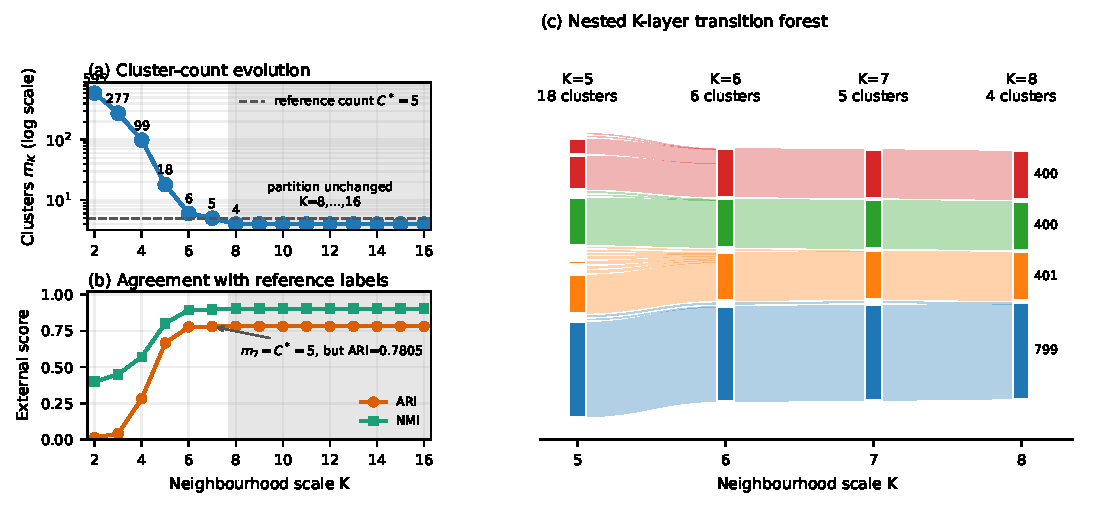
\includegraphics[width=\linewidth]{blobs_var_density_multiscale_transition.pdf}
\caption{Multiscale evolution of the unpruned historical inverse-square model
on the variable-density blobs.  Every layer is generated independently with
$K_0=K$.  (a) The cluster count decreases from 595 microclusters at $K=2$ to
four components at $K=8$ and is plotted on a logarithmic scale; the dashed
line is the reference count $C^*=5$, used only for evaluation.  (b) ARI and
NMI against the withheld reference labels.  The shaded interval marks the
exactly unchanged partition from $K=8$ through the largest tested value,
$K=16$.  (c) The merge-only transition forest over $K=5,6,7,8$.  Node and
ribbon thicknesses encode point population and overlap count
$W_{ab}^{(K,K')}$, respectively.  Colours identify the four lineages ending
at $K=8$ and do not encode reference labels.  The equality $m_7=C^*$ without
high ARI and the stable $m_K=4$ plateau demonstrate that cluster-count or
partition stability alone does not guarantee recovery of latent classes.}
\label{fig:multiscale_transition}
\end{figure}

\section{Scale, popularity, visibility, and saturation}\label{sec:scale}

The formulation suggests an interpretation in terms of propagation, popularity, and selectivity. In the present graph setting, this balance is implemented through the neighbourhood scale $K$, the kernel-dependent reverse-neighbour popularity score $P_{K,g}(x_i)$, and the local visibility threshold $V_{K,g}^{(2)}(x_i)$. Small values of $K$ preserve local selectivity but may fragment the graph. Larger values of $K$ increase propagation, while popularity-modulated RMS visibility prevents all KNN links from being treated as equally admissible.

The base RMS visibility threshold in Eq.~\eqref{eq:rms_visibility_base} acts as a pointwise scale estimate in squared-distance units, while Eq.~\eqref{eq:popularity_modulated_visibility} introduces a popularity-dependent enlargement. In dense regions the base threshold is small and expansion remains selective. Points receiving many influential incoming KNN links obtain higher popularity and may propagate through a larger visible neighbourhood. The kernel determines what constitutes an influential incoming link without changing the closure operator.

The singleton-rejection rule in Eq.~\eqref{eq:singleton_rejection} adds a second selectivity mechanism. A seed that cannot produce a nontrivial saturated closure is not reported as a cluster. Thus, the reported layer is determined not only by reachability in the directed KNN graph, but also by reverse-neighbour popularity, visibility-filtered propagation, and nontrivial closure size.

As $K$ increases, the induced layers may pass from microfragmented local structures to stable macro-scale agglomerations. The saturation scale $K_{\mathrm{sat}}$ provides an empirical way to select the neighbourhood scale from the layer sequence itself, rather than fixing $K$ solely as an external hyperparameter.

\section{Experimental protocol}\label{sec:experimental_protocol}

The controlled benchmark reuses the eight synthetic datasets already distributed with the implementation:
\begin{itemize}
    \item Gaussian blobs with equal and variable densities;
    \item two moons and concentric circles;
    \item anisotropic Gaussian clusters;
    \item a uniform point cloud;
    \item two dense clusters connected by a sparse bridge;
    \item a Swiss-roll embedding.
\end{itemize}
The label column is used only for evaluation and is never included among the clustering features. The Swiss-roll labels are an artificial discretisation of a continuous manifold and its external scores are therefore interpreted descriptively. ARI and NMI are not reported for the uniform dataset because it has no nontrivial reference partition.

For every dataset, $K$ ranges from 2 through 16. Each $K$ is run independently with $K_0=K$. The KNN graph is constructed once for a dataset--$K$ pair and is reused unchanged by all four vote kernels. All models share the inverse-square source budget in Eq.~\eqref{eq:historical_source_budget} and therefore require strictly positive neighbour distances, so the input is checked for exact duplicate points before execution. Uniform, inverse-distance, inverse-square, and sigmoid refer to the four allocation shapes in Eq.~\eqref{eq:vote_kernel_family}; the sigmoid uses $\alpha=8$. RMS visibility and singleton rejection are enabled for every model. Structural pruning is disabled throughout this 840-row comparison, preserving a controlled ablation in which only the within-source allocation changes.

The bridge benchmark varies the retained fraction of the existing labelled bridge points over $\{0,0.10,0.25,0.50,0.75,1\}$. Core points are never subsampled. The two dense cores are considered merged when their dominant predicted cluster identifier is the same; this criterion is independent of the numerical names assigned to clusters.

The output is one long-format CSV. For each dataset, $K$, and vote model, it records:
\begin{itemize}
    \item the dataset name, $K$, vote model, and complete model parameters;
    \item the number of clusters and unclustered points;
    \item ARI and NMI when a nontrivial reference partition is available \citep{HubertArabie1985,VinhEppsBailey2010};
    \item the mean number of visible neighbours and mean visibility in squared-distance units;
    \item end-to-end runtime, including KNN-graph construction;
    \item the bridge-merger indicator for the parameterised bridge rows.
\end{itemize}
The same measured graph-construction time is included in each of the four model runtimes for a given dataset--$K$ pair. This preserves end-to-end interpretation while ensuring that differences in graph construction cannot favour one vote kernel.

Structural pruning is evaluated separately in the native C executable under
the historical inverse-square vote.  Each case is run twice with identical
coordinates and isolated $K$: once with the default unpruned closure and once
with \texttt{--structural-pruning}.  The selected cases are variable-density
blobs at $K=8$, the complete sparse bridge at $K\in\{6,10\}$, and three
preservation controls---circles at $K=7$, two moons at $K=10$, and anisotropic
blobs at $K=8$.  The fixed implementation constants are one through four
diagonal mixture components, five restarts for $m>1$, a minimum BIC gain of
10, the parent and child sizes in Eqs.~\eqref{eq:pruning_parent_size} and
\eqref{eq:pruning_child_size}, and a four-component veto.  The executable is
passed \texttt{--dim 2}; the label column is read only afterwards to compute
ARI and NMI.  Complete native logs, layer files, input hashes, and a
machine-readable parameter manifest accompany the figures.

To test whether the two principal corrections depend on the historical allocation shape,
the variable-density blobs at $K=8$ and the complete bridge at $K=6$ are also
run natively with the three budget-matched shapes $1/u$, $1/u^2$, and
$S_\alpha(u)$, with $\alpha=8$.  Uniform allocation remains in the broader
unpruned ablation but is excluded from this focused weighted-kernel check.  For
each kernel, the C baseline must first match the corresponding Python
partition pointwise; the same native mixture, BIC, size, coherence, and pruning
parameters are then applied without retuning.

\subsection{External-method comparison protocol}

The final comparison uses the six datasets having nontrivial discrete
references and seven external methods: agglomerative clustering, $k$-means,
Gaussian mixtures, DBSCAN, OPTICS, KNN-affinity spectral clustering, and
HDBSCAN.  The uniform cloud has no reference partition, and the Swiss-roll
bands are an artificial discretisation of a continuous manifold; both are
therefore excluded from this table.  No method-specific standardisation is
applied: every method receives the same raw feature columns.

Structurally pruned RTKNNC uses the historical inverse-square vote and sweeps
$K=2,\ldots,16$ in the native executable.  Agglomerative clustering evaluates
Ward, complete, average, and single linkage, both without a connectivity
constraint and with symmetric KNN connectivity at 5, 10, and 15 neighbours.
$k$-means uses 20 initialisations; Gaussian mixtures use five initialisations
under full, tied, diagonal, and spherical covariance models.  These three
methods and spectral clustering receive the reference cluster count $C^*$.
Spectral clustering uses KNN affinity with $k_g=2,\ldots,16$, ARPACK
eigenvectors, and 20 label-assignment restarts at random seed zero.

DBSCAN sweeps $m\in\{3,5,10,20\}$ for \texttt{min\_samples}.  For each $m$,
let $d_i^{(m)}$ be the distance from $x_i$ to its $(m-1)$st proper neighbour,
because DBSCAN counts the query point itself.  Its $\epsilon$ candidates are
the 400 empirical quantiles of $\{d_i^{(m)}\}_{i=1}^N$ at
$q=0.0025,0.005,\ldots,1$.  OPTICS combines the same four values of $m$ with
$\xi\in\{0.01,0.025,0.05,0.1\}$ and minimum-cluster fractions
$\{0.01,0.025,0.05\}$.  HDBSCAN combines minimum cluster sizes
$\{5,10,20,50,100\}$, \texttt{min\_samples} in
$\{\texttt{None},5,10,20\}$, and excess-of-mass or leaf selection.  These
three density-based methods infer their reported cluster counts.

For each method--dataset pair, the table reports the candidate with maximum
ARI, then maximum NMI.  Remaining external-method ties prefer fewer noise
points and then the first candidate in the declared grid; RTKNNC ties prefer
smaller $K$.  Thus, the result is explicitly a label-selected oracle envelope
measuring what each fixed grid can represent, not a claim that ARI supplies an
unsupervised deployment rule.  A noise identifier $-1$ participates in ARI
and NMI as a predicted label, while the reported cluster count excludes it.
The comparison comprises 10,344 external fits and 90 RTKNNC fits.  Complete
external sweeps, selected rows, raw selected labels, software versions, input
hashes, and a provenance-checked table manifest accompany the article
artifacts.

\section{Vote-model benchmark results}\label{sec:vote_results}

The complete sweep contains 840 observations: 480 rows from eight datasets, 15 values of $K$, and four kernels, plus 360 rows from six bridge fractions, 15 values of $K$, and four kernels. No observation contained an unclustered point. Among the 210 matched dataset--scale configurations, the number of clusters differed across kernels in 60 configurations; ARI and NMI differed in 57 labelled configurations. The mean number of visible neighbours and the mean visibility both differed in all 210 configurations. Thus, the allocation shape frequently changes the internal visibility dynamics, although the resulting external optimum can remain stable.

For anisotropic clusters, equal-density blobs, circles, and moons, every kernel attained ARI=NMI=1 within the tested $K$ range. In this unpruned ablation, all kernels also attained the same best result for variable-density blobs (ARI $0.7817$, NMI $0.9035$, $K=8$) and for the labelled bridge dataset (ARI $0.8083$, NMI $0.8182$, $K=6$). These are baseline optima, not the final results of the structural-pruning enhancement reported in Sect.~\ref{sec:structural_pruning_results}. For the discretised Swiss roll, the best scores were low, as expected for an artificial banding of a continuous manifold.  All optima occurred at $K=4$: uniform, inverse-distance, inverse-square, and sigmoid allocation attained ARI/NMI $0.1559/0.5160$, $0.1544/0.5141$, $0.1528/0.5131$, and $0.1558/0.5153$, respectively.

For the coloured comparison figures only, a common representative K is selected
for each labelled dataset by maximising the mean ARI across the four kernels,
with ties resolved in favour of the smaller K.  The same selected K is then
used in every predicted panel, so the graphical comparison does not grant a
different scale to each kernel.  This visualisation rule does not filter the
long-format results, which retain all $K=2,\ldots,16$ observations.

Figure~\ref{fig:moons_vote_models} provides a representative non-convex case in
which all four kernels recover the reference partition exactly.  The more
difficult variable-density case is reserved for the focused, pruned
three-kernel mosaic in Fig.~\ref{fig:blobs_pruning_vote_kernels}.

\begin{figure}[t]
\centering
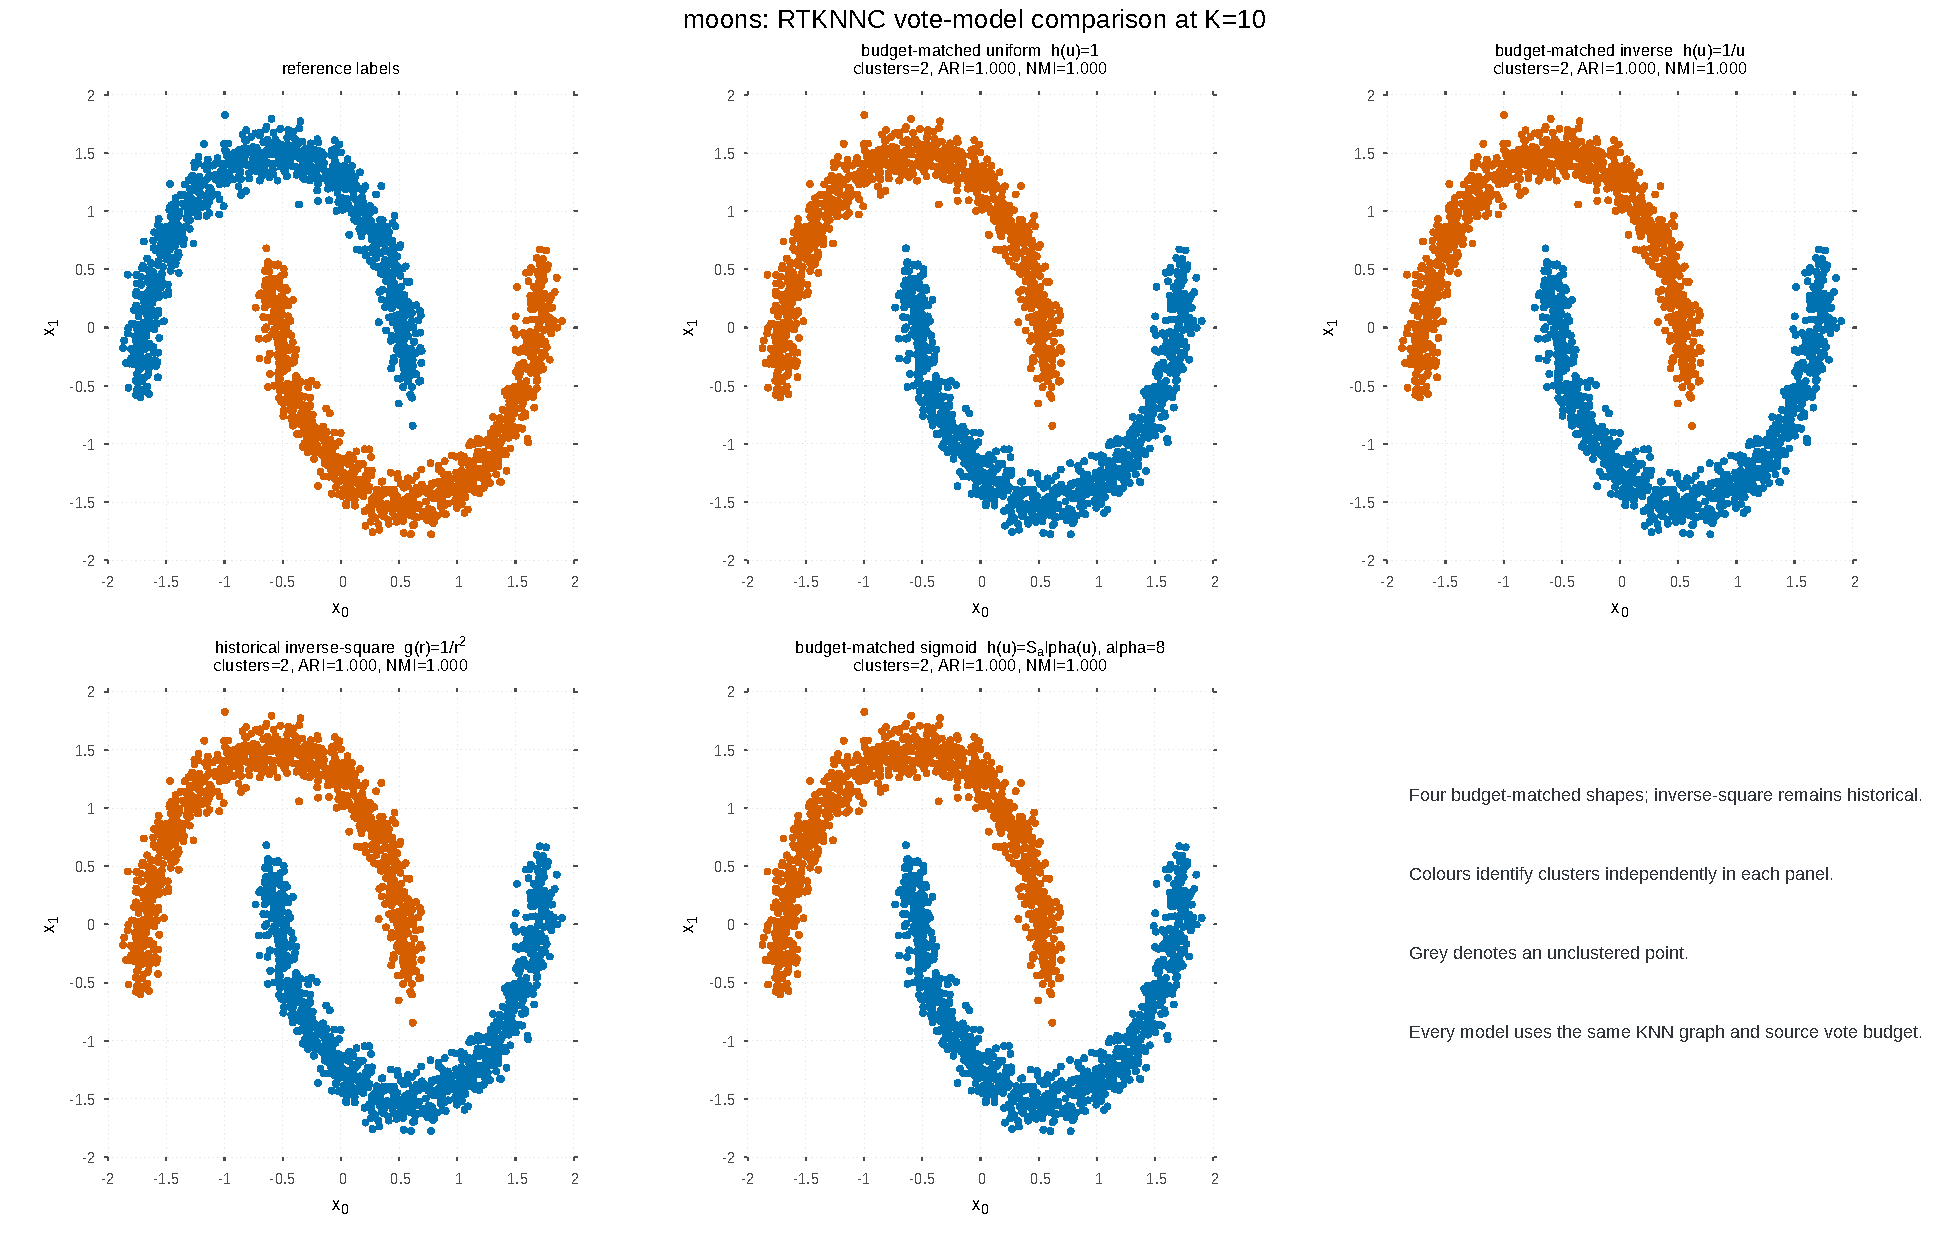
\includegraphics[width=0.98\linewidth]{moons_vote_models_K10_gnuplot.pdf}
\caption{Reference labels and the four predicted partitions for the two-moons
dataset at the common representative scale $K=10$: budget-matched uniform
$h(u)=1$, inverse-distance $h(u)=1/u$, historical inverse-square
$h(u)=1/u^2$, and local sigmoid $S_\alpha(u)$ with $\alpha=8$.  Every source
casts the common budget in Eq.~\eqref{eq:historical_source_budget}; the panels
differ only in its allocation among outgoing neighbours.  Every vote model recovers the two
non-convex components exactly (ARI${}={}$NMI${}={}$1).  The GNUplot rendering
explicitly labels both coordinate axes; cluster colours are local to each
panel and do not encode a cross-panel label correspondence.}
\label{fig:moons_vote_models}
\end{figure}

The cluster count alone can conceal this failure.  At $K=6$, the six reported
components do not include the compact overlapping Gaussian as an independent
cluster: one component contains all 400 of its points together with 390 of the
400 points from the diffuse Gaussian.  The two additional components are small
fragments.  At $K=8$, the merged component contains all 400 compact points and
399 diffuse points.  No tested value $K=2,\ldots,16$ in the \emph{unpruned}
four-kernel sweep recovers the five-class reference partition: smaller $K$
fragments the point cloud before the overlapping distributions separate,
whereas larger $K$ connects them.  This observation diagnoses the connectivity
closure alone; it is precisely the failure corrected by the label-free native
pruning result in Fig.~\ref{fig:blobs_pruning_vote_kernels}.

\subsection{Parameterised bridge transition}

Table~\ref{tab:bridge_transition} reports the first value of $K$ at which the two dense cores share a dominant predicted cluster. No kernel merged the disconnected cores when all bridge points were removed. At bridge fraction $0.10$, the historical inverse-square allocation merges one scale later than the other three; the boundaries coincide at the remaining tested fractions. This is direct evidence that the budget-matched shapes are not equivalent implementations.

\begin{table}[t]
\caption{First $K$ producing a merger of the two dense bridge cores for each of
the four vote kernels. A value $>16$ means that no merger occurred in the
tested range.}\label{tab:bridge_transition}
\centering
\begin{tabular}{rcccc}
\toprule
bridge fraction & $h(u)=1$ & $h(u)=1/u$ & $h(u)=1/u^2$ & $S_\alpha(u)$\\
\midrule
0.00 & $>16$ & $>16$ & $>16$ & $>16$\\
0.10 & 5 & 5 & 6 & 5\\
0.25 & 6 & 6 & 6 & 6\\
0.50 & 6 & 6 & 6 & 6\\
0.75 & 7 & 7 & 7 & 7\\
1.00 & 7 & 7 & 7 & 7\\
\bottomrule
\end{tabular}
\end{table}

For the complete bridge at $K=6$, the two reported components also do not
correspond to the three reference labels.  One contains all 900 points of the
left core, all 200 bridge points, and six peripheral points from the right
core; the other contains the remaining 894 right-core points.  The bridge has
therefore already been absorbed by the left component even though the two dense
cores have not yet fully merged.

\section{Native structural-pruning results}
\label{sec:structural_pruning_results}

Table~\ref{tab:native_structural_pruning} separates the native pruning
experiment from the four-kernel sweep.  The variable-density case changes from
four to five clusters at $K=8$, with ARI increasing from $0.7817$ to $0.9627$.
The accepted split removes 12 crossing visible connections.  The result is not
a relabelling of the reference partition: the five inferred cluster sizes are
$375$, $400$, $400$, $401$, and $424$, so the remaining disagreement is
reported rather than hidden by the correct cluster count.

For the complete sparse bridge, pruning recovers three components at both
tested scales.  At $K=6$, ARI increases from $0.8083$ to $0.9853$ after 10
crossing connections are pruned.  At $K=10$, the unpruned closure has already
collapsed to one component, but a three-child split removes 32 crossing
connections and reaches ARI $0.9865$.  Circles, moons, and anisotropic blobs
serve as preservation controls: no split is accepted, no connection is
removed, and their ARI remains exactly $1$.

\begin{figure}[t]
\centering
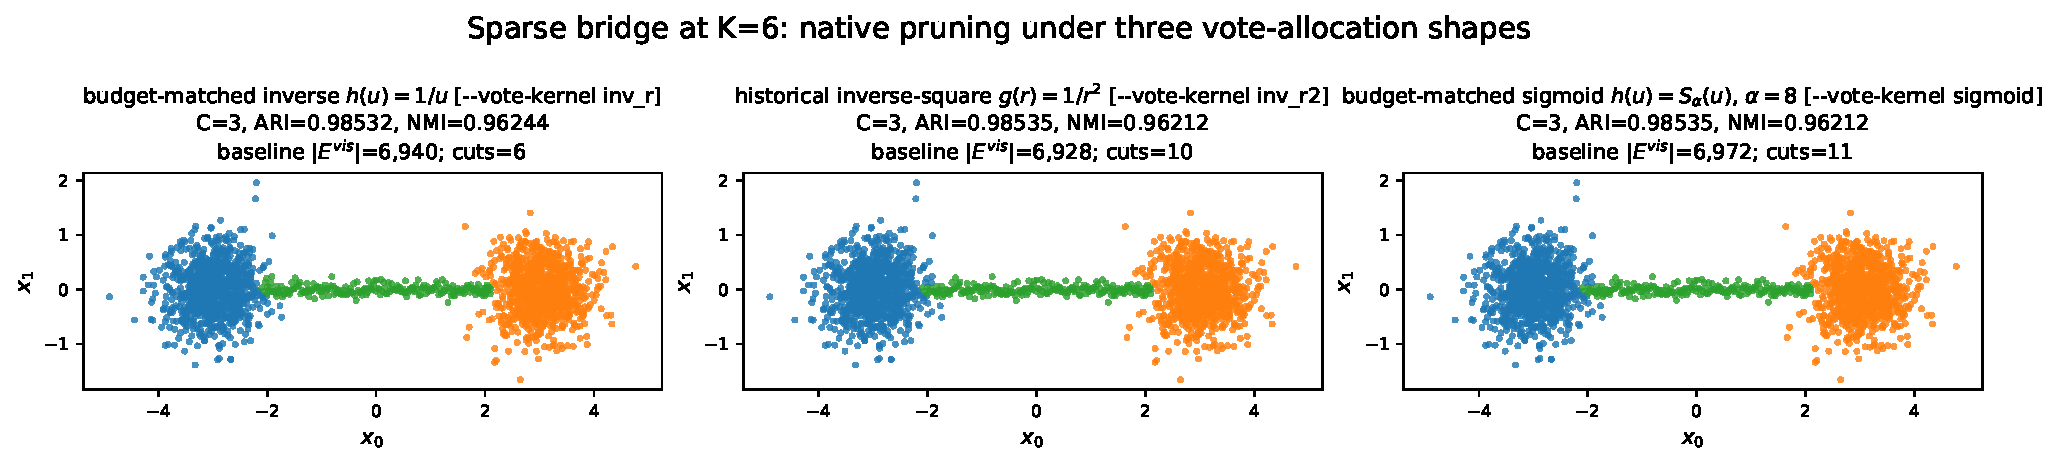
\includegraphics[width=0.98\linewidth]{bridge_native_structural_pruning_vote_kernels_K6.pdf}
\caption{Native structural pruning of the complete sparse bridge at $K=6$
under the three weighted allocation shapes.  The panels show budget-matched
$h(u)=1/u$, historical $h(u)=1/u^2$, and budget-matched local sigmoid
$S_\alpha(u)$ with $\alpha=8$, respectively.  Every model produces three
clusters.  Inverse-square and sigmoid allocation coincide pointwise (ARI
$0.98535$, NMI $0.96212$), while inverse-distance differs from them at four
points after label alignment (ARI $0.98532$, NMI $0.96244$).  The three models
remove 6, 10, and 11 crossing visible connections, and their annotated native
baseline visible-edge counts are 6940, 6928, and 6972, respectively.
Each panel comes from a separate native execution whose recorded command
contains the displayed \texttt{--vote-kernel} token; the equal second and third
scores reflect a pointwise-identical final partition despite distinct baseline
graphs, not reuse of a layer file.
The reference panel is intentionally omitted; reference labels are not
available to the clustering or pruning stages.}
\label{fig:bridge_pruning_vote_kernels}
\end{figure}

\begin{table}[t]
\caption{Native inverse-square baseline and structural-pruning results.  $C^*$
is the number of reference classes, $C_0$ and $C_p$ are the unpruned and pruned
cluster counts, and $|E^{\mathrm{cut}}|$ is the number of crossing visible
connections removed.  Labels are used only for the reported ARI and $C^*$.}
\label{tab:native_structural_pruning}
\centering
\small
\begin{tabular}{lrrrrrrr}
\toprule
dataset & $K$ & $C^*$ & $C_0$ & ARI$_0$ & $C_p$ & ARI$_p$ & $|E^{\mathrm{cut}}|$\\
\midrule
Variable-density blobs & 8 & 5 & 4 & 0.7817 & 5 & 0.9627 & 12 \\
Sparse bridge & 6 & 3 & 2 & 0.8083 & 3 & 0.9853 & 10 \\
Sparse bridge & 10 & 3 & 1 & 0.0000 & 3 & 0.9865 & 32 \\
Circles & 7 & 2 & 2 & 1.0000 & 2 & 1.0000 & 0 \\
Two moons & 10 & 2 & 2 & 1.0000 & 2 & 1.0000 & 0 \\
Anisotropic blobs & 8 & 3 & 3 & 1.0000 & 3 & 1.0000 & 0
\\
\bottomrule
\end{tabular}
\end{table}

\subsection{Pruning sensitivity to the vote kernel}

Figures~\ref{fig:bridge_pruning_vote_kernels} and
\ref{fig:blobs_pruning_vote_kernels} address whether the successful split is
an artefact of the historical inverse-square vote.  For the variable-density
blobs, all three weighted allocation shapes start from four unpruned components and
produce the same five-cluster partition after pruning: ARI $0.9627$, NMI
$0.9614$, and 12 removed connections.  The three partitions are pointwise
identical up to label permutation.  Their mean visible-neighbour counts are
not identical ($4.7010$, $4.6825$, and $4.7350$, respectively), confirming
that the kernels alter the visible graph.  In the companion Python edge audit,
whose partitions pass the native agreement gate, the inverse-square directed
edge set differs from the inverse-distance and sigmoid sets by 89 and 269
visible edges, respectively.  These changes remain inside the same connected
components, and the accepted pruning split therefore coincides at this scale.

The bridge result is also stable in its scientific conclusion.  Every kernel
starts from two components and returns the intended three, with ARI between
$0.98532$ and $0.98535$.  Inverse-square and sigmoid allocation induce the same
partition, while inverse-distance differs by four peripheral assignments after
optimal label alignment.  They remove 10, 11, and 6 crossing connections,
respectively, when listed as inverse-square, sigmoid, and inverse-distance. In
the companion Python edge audit, the inverse-square baseline visible edge set
differs by 56 and 190 directed edges from inverse-distance and sigmoid voting,
respectively.  The equality of cluster counts is
therefore supported by near-identical external partitions, not used as a
substitute for them.

\begin{figure}[t]
\centering
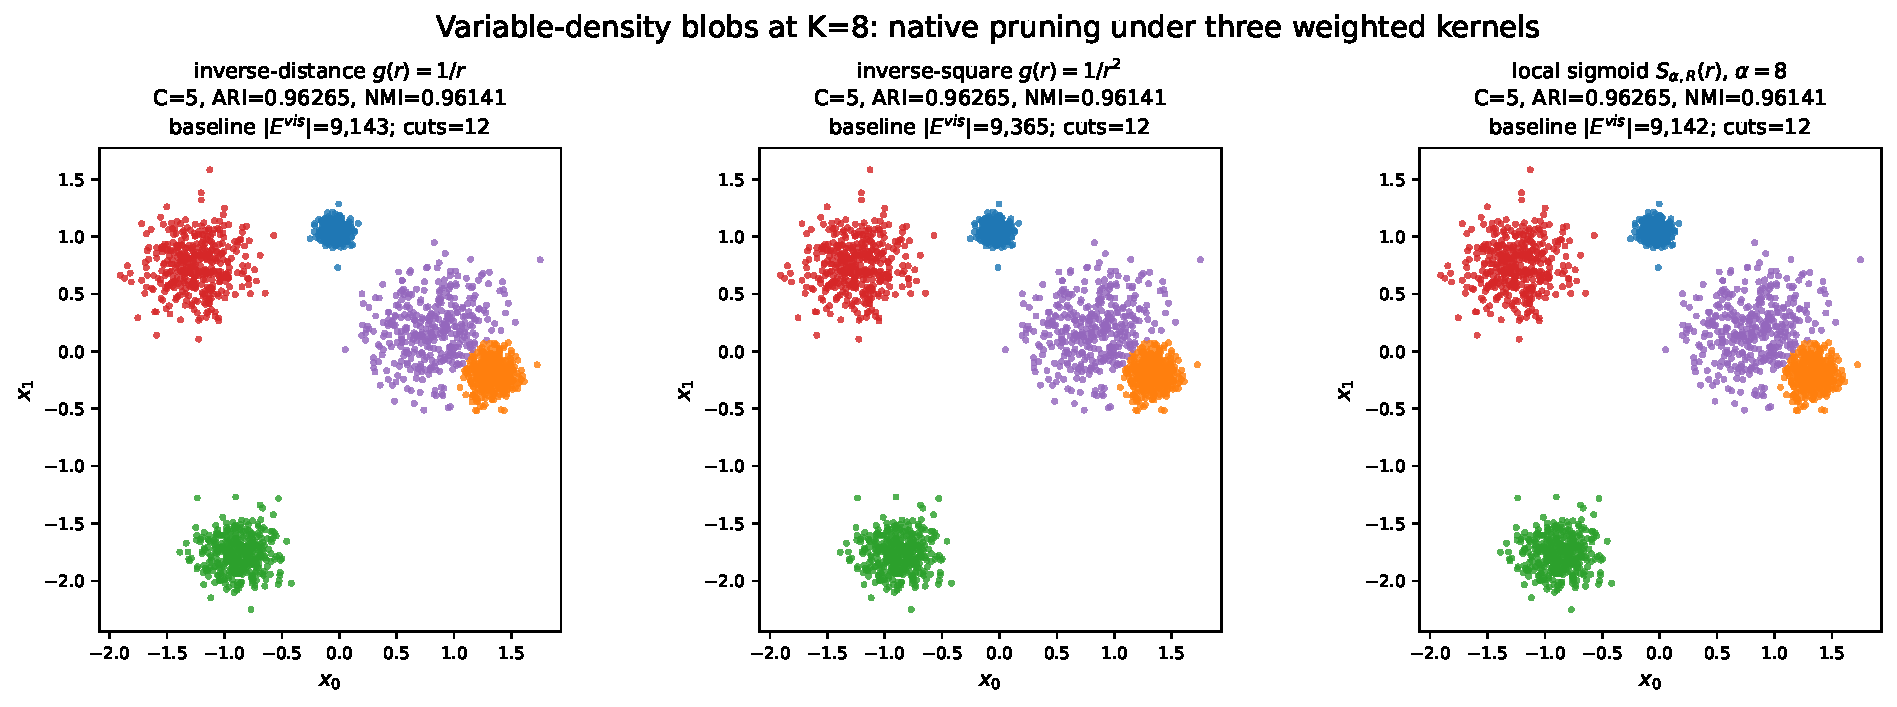
\includegraphics[width=0.98\linewidth]{blobs_var_density_native_structural_pruning_vote_kernels_K8.pdf}
\caption{Native structural pruning of the variable-density blobs at $K=8$
under the three weighted allocation shapes.  The three panels show, from left
to right, budget-matched $h(u)=1/u$, historical $h(u)=1/u^2$, and
budget-matched local sigmoid $S_\alpha(u)$ with $\alpha=8$.  All produce the
same pointwise five-cluster partition (ARI
$0.96265$, NMI $0.96141$) after removing 12 crossing visible connections.
The panel annotations expose the distinct native baseline graphs:
$|E^{\mathrm{vis}}|=9402$, 9365, and 9470 directed edges, respectively.
Reference labels are omitted from the mosaic and are used only for colour
alignment and external scores; each unpruned C partition was first verified
pointwise against its Python kernel definition.}
\label{fig:blobs_pruning_vote_kernels}
\end{figure}

\section{Comparison with external clustering methods}
\label{sec:baseline_comparison}

Table~\ref{tab:all_methods_comparison} reports the oracle envelope defined in
Sect.~\ref{sec:experimental_protocol}.  RTKNNC attains
ARI${}={}$NMI${}={}$1 on anisotropic blobs, equal-density blobs, circles, and
two moons.  Several external methods tie these results, but the controls also
expose their inductive biases: $k$-means and Gaussian mixtures fail on circles
and two moons, whereas graph-, density-, and connectivity-constrained methods
recover the non-convex partitions.  In particular, the degradation of
$k$-means is expected rather than an implementation anomaly.  Its
nearest-centroid assignment induces convex Voronoi cells, which cannot
represent two concentric rings adequately and only approximates the curved,
interleaving moons.  Consequently, it obtains ARI/NMI
$-0.0004/0.0001$ on circles and $0.4800/0.3815$ on two moons.  This limitation
persists even under the favourable protocol used here, in which $k$-means is
given the reference cluster count $C^*=2$.

The two connectivity-stress cases provide finer discrimination.  On the
variable-density blobs, RTKNNC returns the intended five clusters with ARI
$0.9627$ and NMI $0.9614$, narrowly below the full-covariance Gaussian-mixture
result $0.9639/0.9636$.  Spectral clustering reaches $0.9569/0.9581$, while
agglomerative clustering, $k$-means, OPTICS, and HDBSCAN obtain ARIs between
$0.9052$ and $0.9306$.  DBSCAN reaches ARI $0.7916$ and NMI $0.8044$; its
score-maximising candidate fragments the data into 15 clusters and marks 204
points as noise.

On the sparse bridge, RTKNNC attains the highest score,
$0.9865/0.9632$, followed closely by the full-covariance Gaussian mixture at
$0.9831/0.9552$.  Spectral clustering reaches $0.9487/0.8993$, and the other
external ARIs range from $0.6723$ to $0.9342$.  The RTKNNC bridge envelope
selects $K=11$ by a marginal ARI advantage over $K=10$; the focused $K=6$
experiment remains useful because it isolates the earliest corrected
three-component partition under the three vote kernels.

\begin{table*}[t]
\caption{Best label-selected grid result for structurally pruned RTKNNC and
external clustering methods. Each cell reports ARI/NMI; bold denotes the
highest ARI in the row, including ties. Methods marked $\dagger$ receive the
reference cluster count $C^*$; the others do not. Reference labels are used
only for scoring and oracle selection, never as clustering features.}
\label{tab:all_methods_comparison}
\centering
\resizebox{\textwidth}{!}{%
\begin{tabular}{lc*{8}{c}}
\toprule
dataset & $C^*$ & RTKNNC & Agglom.$^\dagger$ & K-means$^\dagger$ & GMM$^\dagger$ & DBSCAN & OPTICS & Spectral$^\dagger$ & HDBSCAN \\
\midrule
Anisotropic & 3 & \textbf{1.0000/1.0000} & \textbf{1.0000/1.0000} & \textbf{1.0000/1.0000} & \textbf{1.0000/1.0000} & \textbf{1.0000/1.0000} & \textbf{1.0000/1.0000} & \textbf{1.0000/1.0000} & \textbf{1.0000/1.0000} \\
Equal-density blobs & 4 & \textbf{1.0000/1.0000} & \textbf{1.0000/1.0000} & \textbf{1.0000/1.0000} & \textbf{1.0000/1.0000} & \textbf{1.0000/1.0000} & 0.9987/0.9977 & \textbf{1.0000/1.0000} & 0.9940/0.9902 \\
Variable-density blobs & 5 & 0.9627/0.9614 & 0.9306/0.9444 & 0.9189/0.9338 & \textbf{0.9639/0.9636} & 0.7916/0.8044 & 0.9266/0.9262 & 0.9569/0.9581 & 0.9052/0.9075 \\
Sparse bridge & 3 & \textbf{0.9865/0.9632} & 0.9153/0.8580 & 0.9342/0.8780 & 0.9831/0.9552 & 0.8140/0.7422 & 0.6723/0.6491 & 0.9487/0.8993 & 0.8641/0.7828 \\
Circles & 2 & \textbf{1.0000/1.0000} & \textbf{1.0000/1.0000} & -0.0004/0.0001 & -0.0004/0.0001 & \textbf{1.0000/1.0000} & \textbf{1.0000/1.0000} & \textbf{1.0000/1.0000} & \textbf{1.0000/1.0000} \\
Two moons & 2 & \textbf{1.0000/1.0000} & \textbf{1.0000/1.0000} & 0.4800/0.3815 & 0.5096/0.4080 & \textbf{1.0000/1.0000} & 0.9990/0.9972 & \textbf{1.0000/1.0000} & \textbf{1.0000/1.0000} \\
\bottomrule
\end{tabular}%
}
\end{table*}


The comparison therefore supports competitiveness rather than universal
superiority.  RTKNNC ties the best result on the standard controls, is within
$0.0013$ ARI of the best variable-density result, and leads on the sparse
bridge.  The fixed-count baselines have the advantage of receiving $C^*$,
whereas RTKNNC and the three density-based methods do not.  Repeated
stochastic realisations, higher-dimensional data, and a label-free
parameter-selection study remain necessary.

\section{Discussion}\label{sec:discussion}

The method should be positioned carefully. It is not a first use of KNN graphs for clustering, nor a replacement for all density-based methods. Its distinctive aspect is the recursive use of forward KNN selection and reverse-neighbour retrieval under a popularity-modulated RMS visibility filter, followed by singleton rejection and saturation analysis. The optional enhancement adds conservative, leadership-seeded structural pruning after closure rather than replacing the graph operator. This places the method between shared-neighbour clustering, reverse-neighbour graph reasoning, closure-based graph clustering, and local model-based partitioning.

The baseline method is an algorithmic and topological construction rather than the minimisation of an explicit objective function. The benchmark supports this distinction: changing only the vote allocation altered the cluster count in 60 of 210 matched configurations and altered visibility in every configuration, yet several datasets shared the same externally optimal partition across all kernels. The allocation shape controls the distribution of incoming evidence, whereas the round-trip graph and its closure determine how visible evidence propagates. Structural pruning is deliberately reported as a separate stage because its BIC criterion introduces an explicit local statistical model.

The inverse-square kernel retains a special implementation-level status: it is
the historical rule and is preserved exactly.  A raw comparison against $1$,
$1/r$, and a bounded sigmoid would, however, mix kernel shape with incompatible
units and outgoing amplitudes; on these data, the raw sigmoid was consequently
almost indistinguishable from uniform voting.  The source-budget-matched family
removes that confound by conserving $B_K(x_i)$ for every source and changing
only how that mass is distributed among its $K$ outgoing edges.  It also makes
$P_{K,g}R_K^{(2)}$ invariant under global coordinate rescaling for every model,
not just inverse-square.  Feature-wise transformations can still change the
neighbour graph, so preprocessing remains part of the method specification.

Within the fixed coordinates of the two difficult cases, however, the pruning
conclusion is not specific to inverse-square voting.  This should not be read
as kernel equivalence.  For the variable-density blobs, the three kernels
produce pointwise-identical final partitions even though their native mean
visible-neighbour counts differ and the companion audit finds hundreds of
kernel-dependent directed edges.  Those edge changes occur within the same
symmetrised connected components, and the mixture stage accepts the same
geometric subdivision.  For the bridge, the stability is only approximate:
inverse-distance voting changes four assignments relative to the pointwise-
identical inverse-square and sigmoid results, a distinction hidden by
three-decimal ARI and NMI.  Thus,
the matching blob scores identify an empirical topological stability plateau,
not redundant kernel implementations, while the bridge demonstrates that
small kernel effects remain measurable.  This does not establish general
kernel invariance; it shows that the reported correction survives the most
immediate alternative-kernel challenge without retuning the pruning rule.

The bridge result should also be interpreted narrowly.  At retained bridge
fraction $0.10$, uniform, inverse-distance, and sigmoid allocation first merge
the dense cores at $K=5$, whereas historical inverse-square first merges them
at $K=6$.  This observed boundary difference confirms that equal results at
the complete-bridge reference scale do not imply kernel equivalence.  A denser
sweep over bridge geometry, noise, separation, and sigmoid slope may expose
further transition differences.

\subsection{Connectivity failure and structural correction}

The observed failures follow from the topology of the closure operator.  For a
fixed $K$ and vote kernel $g$, define the visible directed edge set
\begin{equation}
E^{\mathrm{vis}}_{K,g}=\left\{(i,j):
x_j\in\calN_K^+(x_i),\ D_{ij}\leq V_{K,g}^{(2)}(x_i)\right\}.
\label{eq:visible_edge_set}
\end{equation}
Forward expansion traverses outgoing edges in this graph and backward
expansion traverses incoming edges.  Consequently, apart from the explicit
singleton policy, the \emph{unpruned} saturated closures are the connected
components obtained after disregarding the orientation of the visible edges.
The baseline can therefore recover a reference partition exactly only at a
scale for which its classes form separate components of this symmetrised
visible graph.  The enhanced method relaxes that restriction in a controlled
way: Eqs.~\eqref{eq:pruning_acceptance}--\eqref{eq:pruning_cut} permit a large
component to be divided only when independent mixture and graph-coherence
tests agree.

This condition explains why nonconvexity itself is not fatal.  Moons and
circles are nonconvex, but a geometric gap prevents visible paths between their
reference components at an appropriate value of $K$.  The variable-density
example is different: the compact and diffuse right-hand Gaussians overlap in
the same region of the observed space.  Cross-class nearest-neighbour edges are
then unavoidable, and one admissible chain places both latent classes in the
same baseline closure.  Decreasing $K$ removes edges but first produces
microclusters; increasing $K$ strengthens the connection.  Structural pruning
supplies the missing modelling assumption locally: at $K=8$, BIC supports a
two-population subdivision of the merged closure and the visible graph supports
both children.  This recovers five clusters with ARI $0.9627$, while the
residual error appropriately reflects that overlapping coordinates do not
define a uniquely perfect latent boundary.

The sparse bridge creates the analogous phenomenon through a filament rather
than direct overlap.  Its left endpoint reaches vertices that already belong
to the giant left-core component, whereas the closest right-end vertices remain
in small peripheral components until the next scale.  Once a visible path
reaches a giant component, recursive forward--backward expansion absorbs the
entire path; a single cross-boundary connection is sufficient in the baseline.
The native stage identifies three supported populations and prunes 10 crossing
connections at $K=6$, preserving the bridge as a third structure with ARI
$0.9853$.  The Swiss roll presents the complementary case: its reference bands
discretise one continuous manifold, so selective visibility yields many local
components rather than the prescribed bands, while less selective scales
eventually connect across them.  The four-component veto and graph-coherence
test are intended to protect such curved or fragmented structures, but a
systematic manifold study remains necessary.

Thus, the baseline output is a partition of visible KNN connectivity, whereas
the enhanced output is that partition after a conservative local model-based
test of its large components.  Neither is guaranteed to reconstruct every
externally supplied label partition.  The distinction matters scientifically:
the four-kernel sweep measures vote sensitivity of the original closure, while
the native comparison measures the incremental effect of structural pruning.

The present study has several limitations:
\begin{enumerate}
    \item the synthetic results use one deterministic realisation of each dataset family;
    \item the sigmoid experiment fixes $\alpha=8$ rather than sweeping its slope, and the focused three-kernel pruning comparison is restricted to the two difficult reference cases;
    \item the bridge benchmark varies bridge density but not width, curvature, core separation, or noise;
    \item the pruning thresholds and diagonal-covariance family are fixed and have been evaluated here on six primary dataset--scale cases;
    \item overlapping latent classes may remain only approximately identifiable, and broader tests are needed to quantify false splits on curved, heavy-tailed, and high-dimensional data;
    \item the empirical runtime measurements are not a substitute for a formal complexity analysis;
    \item the external comparison uses one implementation and one deterministic realisation of six two-dimensional datasets; it uses reference labels to select every grid optimum and supplies $C^*$ to four fixed-count baselines, so label-free selection, repeated realisations, and comparisons with SNN and mutual-KNN methods remain open.
\end{enumerate}

\section{Conclusion}\label{sec:conclusion}

We presented a clustering method based on popularity-modulated,
visibility-filtered round-trip closure in directed KNN graphs, separated its
topological operator from four source-budget-matched vote-allocation shapes,
preserved the historical inverse-square rule exactly, and added optional native
structural pruning for overly connected closures.  A 120-case inverse-square
C--Python agreement test served as a software regression gate, and the
unpruned 840-row sweep showed that the kernel often changes visibility and
sometimes the induced partition.  The native enhancement then corrected the
central connectivity failures: variable-density blobs changed from four to
five clusters with ARI $0.7817\to0.9627$, and the bridge reached three clusters
with ARI $0.9853$ at $K=6$ and $0.9865$ at $K=10$.  It accepted no split on
three already correct controls, whose ARI remained $1$.  At the two difficult
reference scales, inverse-distance, inverse-square, and sigmoid voting all
preserved the corrected cluster counts with essentially identical scores, and
their six unpruned native partitions passed pointwise C--Python agreement.
A 10,434-candidate oracle-envelope comparison with seven external methods then
showed that pruned RTKNNC ties the perfect result on the standard controls,
nearly matches the best variable-density result ($0.9627$ versus $0.9639$ for
a full-covariance Gaussian mixture), and attains the highest sparse-bridge ARI
($0.9865$).  These results show that vote weighting, visible connectivity, and
structural correction are distinct experimental axes.  Broader replication is
still required for the fixed pruning thresholds, high-dimensional data,
alternative covariance models, label-free scale selection, and additional
graph-based baselines.

\backmatter

\bmhead{Acknowledgements}
To be completed.

\bmhead{Declarations}
\begin{itemize}
\item Funding: To be completed.
\item Conflict of interest/Competing interests: The authors declare that they have no competing interests. To be confirmed.
\item Ethics approval and consent to participate: Not applicable.
\item Consent for publication: Not applicable.
\item Data availability: Synthetic datasets and scripts will be made available in a public repository upon publication. To be completed.
\item Materials availability: Not applicable.
\item Code availability: The implementation will be made available in a public repository upon publication. To be completed.
\item Author contribution: To be completed.
\end{itemize}

\bibliography{round_trip_knn_nca_sn_draft_popularity_visibility}

\end{document}
